\documentclass[
  10pt,       % fontsize
  twoside,    % symmetric pagination, for digital view
  % oneside,  % asymmetric pagination, for a nice printed version
  a4paper,    % 
  english,    % 
  tikz,       % to build images
  openright,  % start chapters on odd-numbered pages
]{book}

\usepackage{preamble}
\usepackage{graphicx}
\graphicspath{ {./images/} }

\begin{document}

%% config && title page
\frontmatter
%!TEX root = ../dissertation.tex

\newcommand{\myName}{Alessio Ferrarini}
\newcommand{\myTitle}{Abstract Hoare logic}
\newcommand{\myDegree}{Master degree thesis}
\newcommand{\myUni}{University of Padova}
\newcommand{\myFaculty}{Master degree in Computer Science}
\newcommand{\myDepartment}{Department of Mathematics ``Tullio Levi-Civita''}
\newcommand{\profTitle}{Prof.}
\newcommand{\myProf}{Francesco Ranzato}
\newcommand{\myCoProf}{Paolo Baldan}
\newcommand{\myLocation}{Padova}
\newcommand{\myAA}{2023--2024}
\newcommand{\myTime}{April}

\title{\myTitle}
\author{\myName}

% PDF file metadata fields
% when updating them delete the build directory, otherwise they won't change
\begin{filecontents*}{\jobname.xmpdata}
  \Title{Abstract Hoare logic}
  \Author{Alessio Ferrarini}
  \Language{en-EN}
  \Subject{Software Verification}
  \Keywords{Hoare Logic\sep Software Verification\sep Abstract Interpretation}
\end{filecontents*}

% IMPORTANT: Update the metadata!! Contains the subject and the
% keywords

% Author in metadata must be specified again, otherwise it won't
% compile

\begin{titlepage}
  \begin{center}

    \begin{figure}[htbp]
      \centering
      \includegraphics[height=3cm]{unipd-logo}
    \end{figure}

    \vbox to0pt{
      \vbox to\textheight{
        \vfill \includegraphics[width=11.5cm]{unipd-light}
        \vfill}
      \vss}

    \begin{huge}
      \textbf{\myUni}\\
    \end{huge}

    \line(1, 0){\textwidth} \\
    
    \begin{Large}
      \textsc{\myDepartment}\\
    \end{Large}
    
    \vspace{10pt}
    
    \begin{large}
      \textsc{\myFaculty}\\
    \end{large}

    \vspace{30pt}

    \begin{LARGE}
      {\color{unipdred}\textbf{\myTitle}}\\
    \end{LARGE}

    %% \vspace{40pt}
    \vfill

    \begin{large}
      \begin{flushleft}
        \textit{Supervisor}\\
        \vspace{5pt}
        \profTitle\ \myProf\\
        \vspace{20pt}
        \textit{Co. Supervisor}\\
        \vspace{5pt}
        \profTitle\ \myCoProf\\
      \end{flushleft}

      % You can tweak the spacing to have professor and student names on the same line
      % useful if the page is broken by a long thesis title and you need more space
      \vspace{-55pt}

      \begin{flushright}
        \textit{Candidate}\\
        \vspace{5pt}
        \myName
      \end{flushright}
    \end{large}

    %% \vspace{40pt}

    \line(1, 0){\textwidth} \\
    \begin{normalsize}
      \textsc{Academic Year \myAA}
    \end{normalsize}
  \end{center}
\end{titlepage}
\cleardoublepage
\phantomsection
\pdfbookmark{Abstract}{Abstract}
\begingroup

\chapter*{Abstract}

In theoretical computer science, program logics are essential for verifying the
correctness of software. Hoare logic provides a systematic way of reasoning
about program correctness using preconditions and postconditions. This thesis
explores the development and application of an abstract Hoare logic framework
that generalizes traditional Hoare logic by using arbitrary elements of
complete lattices as the assertion language, extrapolating what makes Hoare
logic sound and complete. We also demonstrate the practical applications of
this framework by obtaining a program logic for hyperproperties, highlighting
its versatility and benefits. From the design of Abstract Hoare logic, we
define Reverse Abstract Hoare logic, which is used to develop systems for
backward correctness reasoning on programs.

\vfill
\cleardoublepage
\phantomsection
\pdfbookmark{Acknowledgments}{Acknowledgments}

\begingroup

\chapter*{Acknowledgments}

To \dots

\begin{textblock}{1}[1,1](9,10)
  \epigraph{\textit{``Progress is possible only if we train ourselves to think 
  about programs without thinking of them as pieces of executable code.``}}
  {Edsger W. Dijkstra}
\end{textblock}


\endgroup
\cleardoublepage

%% TOC
\cleardoublepage

\begingroup
\hypersetup{linkcolor=black}
\tableofcontents
\endgroup

%% Structure
\cleardoublepage
\mainmatter
% This file only puropouse is to organize the chapters

% import the mod file from each directory, it will tell how the
% chapter is organized
\chapter*{Introduction}

The verification of program correctness is a critical and crucial task in
computer science. Ensuring that software behaves as expected under all possible
conditions is fundamental in a society that increasingly relies on computer
programs. Software engineers often reason about the behavior of their programs
at an intuitive level. While this is definitely better than not reasoning at
all, intuition alone becomes insufficient as the size of programs grows.

Writing tests for programs is definitely a useful task, but at best, it can
show the presence of bugs, not prove their absence. We cannot feasibly write
tests for every possible input of the program. To offer a guarantee of the
absence of undesired behaviors, we need sound logical models rooted in logic.
The field of formal methods in computer science aims at developing the logical
tools necessary to prove properties of software systems.

Hoare logic, first introduced by Hoare in the late 60s \cite{Hoare69}, provides
a set of logical rules to reason about the correctness of computer programs.
Hoare logic formalizes, with axioms and inference rules, the relationship
between the initial and final states after executing a program.

Hoare logic, beyond being one of the first program logics, is arguably also one
of the most influential ideas in the field of software verification. It created
the whole field of program logics—systems of logical rules aimed at proving
properties of programs. Over the years, modifications of Hoare logic have been
developed, sometimes to support new language features such as dynamic memory
allocation and pointers, or to prove different properties such as equivalence
between programs or properties of multiple executions. Every time Hoare logic
is modified, it is necessary to prove again that the proof system indeed proves
properties about the program (soundness) and ideally that the proof system is
powerful enough to prove all the properties of interest (completeness).

Most modifications of Hoare logic usually do not alter the fundamental proof
principles of the system. Instead, they often extend the assertion language to
express new properties and add new commands to support new features in
different programming languages.

In this work, we introduce Abstract Hoare Logic, which aims to be a framework
general enough to serve as an extensible platform for constructing new
Hoare-like logics without the burden of proving soundness and completeness
anew. We demonstrate, through examples, how some properties that are not
expressible in standard Hoare logic can be simply instantiated within Abstract
Hoare Logic, while keeping the proof system as simple as possible.

The theory of Abstract Hoare Logic is deeply connected to the theory of
abstract interpretation \cite{Cousot77}. The semantics of the language is
defined as an inductive abstract interpreter, and the validity of the Abstract
Hoare triples depends on it. Since we do not use the strongest postcondition
directly, we are able to reason about properties that are not expressible in
the powerset of the program states, such as hyperproperties.

This thesis is structured as follows:
\begin{itemize}
  \item In Chapter 1, we introduce the basic mathematical background of order
    theory and abstract interpretation.

  \item In Chapter 2, we introduce standard Hoare logic and the general
    framework of Abstract Hoare Logic: the extensible language $\lang$, its
    syntax and semantics, the generalization of the strongest postcondition,
    and finally, Abstract Hoare Logic and its proof system, proving the general
    results of soundness and relative completeness.

  \item In Chapter 3, we show some notable instantiations of Abstract Hoare
    Logic: we demonstrate that it is possible to obtain program logics where
    the implication is decidable, thus making the goal of checking a derivation
    computable; we show how to obtain a proof system for hyperproperties (and
    we introduce the concept of the strongest hyper postcondition); Finally, we
    show that it is possible to obtain a proof system for partial
    incorrectness.

  \item In Chapter 4, we show how to enrich the barebones proof system of
    Abstract Hoare Logic by adding more restrictions on the assertion language
    or the semantics.

  \item In Chapter 5, we show how to reuse the idea of Abstract Hoare Logic to
    generalize proof systems for backward reasoning.

  \item In Chapter 6, we provide a brief summary of the most important
    contributions of the thesis. We discuss possible extensions to the
    framework of Abstract Hoare Logic and, to conclude, we examine the
    relationship of Abstract Hoare Logic with other similar work.
\end{itemize}

\chapter{Background}

\section{Order theory}\label{sec:backround:order_theory}

When defining the semantics of programming languages, the theory of 
\textit{partially ordered sets} and \textit{lattices} is fundamental
\cite{Gratzer11, Birkhoff40}. These 
concepts are at the core of denotational semantics \cite{Scott70} and 
\textit{Abstract Interpretation} \cite{Cousot77}, where the semantics of 
programming languages and abstract interpreters are defined as monotone 
functions over some complete lattice.

\subsection{Partial Orders}

\begin{definition}[Partial order]
  A partial order on a set $X$ is a relation $\leq \subseteq X \times X$ 
  such that the following properties hold:
  \begin{itemize}
    \item Reflexivity: $\forall x \in X, \; (x, x) \in \; \leq$
    \item Anti-symmetry: $\forall x, y \in X, \; (x, y) \in \; \leq \mand
      (y, x) \in \; \leq \implies x = y$
    \item Transitivity: $\forall x, y, z \in X, \; (x, y) \in \; \leq \mand 
      (y, z) \in \; \leq \implies (x, z) \in \;\leq$
  \end{itemize}
    
\end{definition}

Given a partial order $\leq$, we will use $\geq$ to denote the converse 
relation $\{ (y, x) \mid (x, y) \in \;\leq \}$ and $<$ to denote 
$\{ (x, y) \mid (x, y) \in \;\leq \; \text{and} \; x \neq y \}$.

From now on we will use the notation $x R y$ to indicate $(x, y) \in R$.

\begin{definition}[Partially ordered set]
  A partially ordered set (or poset) is a pair $(X, \leq)$ in which $\leq$ is a 
  partial order on $X$.
\end{definition}

\begin{definition}[Monotone function]
  Given two ordered sets $(X, \leq)$ and $(Y, \sqsubseteq)$, a function 
  $f : X \to Y$ is said to be monotone if $x \leq y \implies f(x) \sqsubseteq 
  f(y)$.
\end{definition}

\begin{definition}[Galois connection]
  Let $(C, \sqsubseteq)$ and $(A, \leq)$ be two partially ordered sets, a 
  Galois connection written $\langle C, \sqsubseteq \rangle 
  \galois{\alpha}{\gamma} \langle A, \leq \rangle$, are a pair of functions:
  $\gamma : A \to D$ and $\alpha : D \to A$ such that:
  \begin{itemize}
    \item $\gamma$ is monotone
    \item $\alpha$ is monotone
    \item $\forall c \in C$ $c \sqsubseteq \gamma(\alpha(c))$
    \item $\forall a \in A$ $a \leq \alpha(\gamma(a))$
  \end{itemize}
\end{definition}

\begin{definition}[Galois Insertion]
  Let $\langle C, \sqsubseteq \rangle \galois{\alpha}{\gamma} \langle A, \leq 
  \rangle$, be a Galois connection, a Galois insertion written 
  $\langle C, \sqsubseteq \rangle \galoiS{\alpha}{\gamma} \langle A, \leq \rangle$
  are a pair of functions: $\gamma : A \to D$ and $\alpha : D \to A$ such that:
  \begin{itemize}
    \item $(\gamma, \alpha)$ are a Galois connection
    \item $\alpha \circ \gamma = id$
  \end{itemize}
\end{definition}

\begin{definition}[Fixpoint]
  Given a function $f : X \to X$, a fixpoint of $f$ is an element $x \in X$ 
  such that $x = f(x)$.

  We denote the set of all fixpoints of a function as $\fix(f) = 
  \{ x \mid x \in X \mand x = f(x) \}$.
\end{definition}

\begin{definition}[Least and Greatest fixpoints]
  Given a function $f : X \to X$,
  \begin{itemize}
    \item We denote the \textit{least fixpoint} as $\lfp(f)$ and is defined as
      $lfp(f) = a^* \in \fix(f)$ and $\forall a \in \fix(f) \; a^* \leq a$.
    \item We denote the \textit{greatest fixpoint} as $\gfp(f)$ and is defined as
      $gfp(f) = a^* \in \fix(f)$ and $\forall a \in \fix(f) \; a^* \geq a$.
  \end{itemize}
\end{definition}

\subsection{Lattices}

\begin{definition}[Meet-semilattice]
  A meet-semilattice is a partially ordered set \((L, \leq)\) such that for
  every pair of elements \(a, b \in L\), there exists an element \(c \in L\)
  satisfying the following conditions: 
  \begin{enumerate}
    \item \(c \leq a\) and \(c \leq b\) 
    \item \(\forall d \in L\), if \(d \leq a\) and \(d \leq b\), then \(d \leq c\) 
\end{enumerate}
  The element \(c\) is called the \emph{meet} of \emph{greatest lower bound} of
  \(a\) and \(b\), and is denoted by \(a \wedge b\).
\end{definition}

\begin{definition}[Join-semilattice]
  A join-semilattice is a partially ordered set \((L, \leq)\) such that for
  every pair of elements \(a, b \in L\), there exists an element \(c \in L\)
  satisfying the following conditions: 
  \begin{enumerate}
    \item \(c \geq a\) and \(c \geq b\) 
    \item \(\forall d \in L\), if \(d \geq a\) and \(d \geq b\), then \(d \geq c\) 
\end{enumerate}
  The element \(c\) is called the \emph{join} or \emph{least upper bound} of
  \(a\) and \(b\), and is denoted by \(a \join b\).
\end{definition}

\begin{observation}
  Both join and meet operations are idempotent, associative, and commutative.
\end{observation}

\begin{definition}[Lattice]
  A poset $(L, \leq)$ is a lattice if it is both a join-semilattice and a 
  meet-semilattice.
\end{definition}

\begin{definition}[Complete lattice]
  A partially ordered set \((L, \leq)\) is called a \emph{complete lattice} if
  for every subset \(S \subseteq L\), there exist elements \(\sup S\) and
  \(\inf S\) in \(L\) such that: 
  \begin{enumerate}
    \item \(\sup S\) (the supremum or least upper bound of \(S\)) is an
      element of \(L\) satisfying: 
      \begin{itemize}
        \item For all \(s \in S\), \(s \leq \sup S\).
        \item For any \(u \in L\), if \(s \leq u\) for all \(s \in S\), then
          \(\sup S \leq u\). \end{itemize}
    \item \(\inf S\) (the infimum or greatest lower bound of \(S\)) is an
      element of \(L\) satisfying: 
      \begin{itemize}
        \item For all \(s \in S\), \(\inf S \leq s\).
        \item For any \(l \in L\), if \(l \leq s\) for all \(s \in S\), then
          \(l \leq \inf S\). 
      \end{itemize}
  \end{enumerate}

  We denote the \textit{least element} or \textit{bottom} as $\bot = \inf \; L$ 
  and the \textit{greatest element} or \textit{top} as $\top = \sup \; L$.
\end{definition}

\begin{observation}
  A complete lattice cannot be empty.
\end{observation}

\begin{definition}[Point-wise lifting]
  Given a complete lattice $L$ and a set $A$ we call \textit{point-wise} lifting
  of $L$ the set of all functions $A \to L$ ordered as follows: $f \sqsubseteq 
  g \iff \forall a \in A \; f(a) \leq f(g)$.
\end{definition}

\begin{observation}[Point-wise fixpoint]
  \label{th:pointfix}
  The least-fixpoint and greatest fixpoint on some point-wise lifted lattice on 
  a monotone function defined point-wise is the point-wise lift of the function.

  $$\lfp(\lambda p' a . f(p'(a))) = \lambda a . \lfp(\lambda p' . f(a))$$
  $$\gfp(\lambda p' a . f(p'(a))) = \lambda a . \gfp(\lambda p' . f(a))$$
\end{observation}

\begin{theorem}[Knaster-Tarski theorem]
  \label{thm:knaster}
  Let $(L, \leq)$ be a complete lattice and let $f : L \to L$ be a monotone 
  function. Then $(\text{fix}(f), \leq)$ is also a complete lattice.
\end{theorem}

We have two direct consequences: both the greatest and the least fixpoint of
$f$ exists as they are respectively top and bottom of $\fix(f)$.

\begin{theorem}[Post-fixpoint inequality]
  \label{thm:post-lfp}
  Let $f$ be a monotone function on a complete lattice then
  $$f(x) \leq x \implies \lfp(f) \leq x$$
\end{theorem}
\begin{proof}
  By theorem \ref{thm:knaster} $\lfp(f) = \bigwedge\{ y \mid y \geq f(y) \}$
  thus $\lfp(f) \leq x$ since $x \in \{ y \mid y \geq f(y) \}$.
\end{proof}

\begin{theorem}[$\lfp$ monotonicity]
  \label{thm:lfp-mono}
  Let $L$ be a complete lattice, if $P \leq Q$ and $f$ is monotone then
  $$\lfp(\lambda X. P \join f(X)) \leq \lfp(\lambda X. Q \join f(X))$$
\end{theorem}
\begin{proof}
  \begin{align*}
    P \join f(\lfp(\lambda X . Q \join f(X)))
      &\leq Q \join f(\lfp(\lambda X . Q \join f(X)))
      &\text{[Since $P \leq Q$]} \\
      &= \lfp(\lambda X . Q \join f(X))
      &\text{[By definition of fixpoint]} \\
  \end{align*}
  Thus by theorem \ref{thm:post-lfp} pick $f = \lambda X . P \join f(X)$ and
  $x = \lfp(\lambda X. Q \join f(X))$ it follows that
  $\lfp(\lambda X. P \join f(X)) \leq \lfp(\lambda X. Q \join f(X))$.
\end{proof}

\section{Abstract Interpretation}

Abstract interpretation \cite{Cousot77, Cousot21} is the de-facto standard
approach for designing static program analysis. The specification of a program
can be expressed as a pair of initial and final sets of states, $Init, Final
\in \pow{\states}$, and the task of verifying a program $C$ boils down to
checking if $\sem{C}(Init) \subseteq Final$.

Clearly, this task cannot be performed in general. The solution proposed by the
framework of abstract interpretation is to construct an approximation of
$\sem{\cdot}$, usually denoted by $\sem{\cdot}^\#$, that is computable.

\subsection{Abstract Domains}

One of the techniques used by abstract interpretation to make the problem of 
verification tractable involves representing collections of states with a finite 
amount of memory.

\begin{definition}[Abstract Domain]
  A poset $(A, \leq)$ is an abstract domain if there exists a Galois insertion
  $\langle \pow{\states}, \subseteq \rangle \galoiS{\alpha}{\gamma} \langle A, 
  \leq \rangle$.
\end{definition}

\begin{example}[Interval Domain]
  \label{exmp:interval}
  Let $Int = \{ [a, b] \mid a, b \in \mathbb{Z} \cup \{+\infty, -\infty \}, a 
  \leq b \} \cup \{ \bot \}$ be ordered by inclusion, each element $[a, b]$ 
  represent the set $\{ x \mid a \leq x \leq b \}$ and $\bot$ is used as a 
  representation of $\emptyset$. The structure of the 
  lattice can be summarized by the following Hasse diagram:

  \begin{center}
  \begin{tikzpicture}[scale=0.9]
    \node [] (0) at (0, 0) {$\bot$};
    \node [] (1) at (0, 1) {$[0, 0]$};
    \draw (0) to (1);
    \node [] (2) at (2, 1) {$[+1, +1]$};
    \draw (0) to (2);
    \node [] (3) at (4, 1) {$[+2, +2]$};
    \draw (0) to (3);
    \node [] (4) at (-2, 1) {$[-1, -1]$};
    \draw (0) to (4);
    \node [] (5) at (-4, 1) {$[-2, -2]$};
    \draw (0) to (5);


    \node [] (c1) at (+6, 1) {\color{black!30}$\dots$};
    \node [] (c2) at (-6, 1) {\color{black!30}$\dots$};
    
    \node [] (6) at (-3, 2) {$[-2, -1]$};
    \draw (5) to (6);
    \draw (4) to (6);
    
    \node [] (7) at (-1, 2) {$[-1, -0]$};
    \draw (4) to (7);
    \draw (1) to (7);
    
    \node [] (8) at (+1, 2) {$[0, 1]$};
    \draw (2) to (8);
    \draw (1) to (8);
    
    \node [] (9) at (+3, 2) {$[1, 2]$};
    \draw (2) to (9);
    \draw (3) to (9);

    \node [] (10) at (-2, 3) {$[-2, 0]$};
    \draw (10) to (6);
    \draw (10) to (7);
    
    \node [] (11) at (0, 3) {$[-1, +1]$};
    \draw (11) to (7);
    \draw (11) to (8);
    
    \node [] (12) at (2, 3) {$[0, +2]$};
    \draw (12) to (8);
    \draw (12) to (9);
    
    \node [] (13) at (-1, 4) {$[-2, +1]$};
    \draw (13) to (10);
    \draw (13) to (11);

    \node [] (14) at (1, 4) {$[-1, +2]$};
    \draw (14) to (11);
    \draw (14) to (12);
    
    \node [] (15) at (0, 5) {$[-2, +2]$};
    \draw (13) to (15);
    \draw (14) to (15);

    \node [] (16) at (-7, 3) {$[-\infty, -2]$};
    \node [] (17) at (-6, 4) {$[-\infty, -1]$};
    \draw (16) to (17);
    \node [] (18) at (-5, 5) {$[-\infty, 0]$};
    \draw (17) to (18);

    \node [] (b1) at (-4, 4) {};
    \draw [loosely dotted] (b1) to (18);
    \node [] (b2) at (-5, 3) {};
    \draw [loosely dotted] (b2) to (17);
    \node [] (b3) at (-6, 2) {};
    \draw [loosely dotted] (b3) to (16);
    
    \node [] (19) at (+7, 3) {$[+2, +\infty]$};
    \node [] (20) at (+6, 4) {$[+1, +\infty]$};
    \draw (19) to (20);
    \node [] (21) at (+5, 5) {$[0, +\infty]$};
    \draw (20) to (21);


    \node [] (a1) at (+4, 4) {};
    \draw [loosely dotted] (a1) to (21);
    \node [] (a2) at (+5, 3) {};
    \draw [loosely dotted] (a2) to (20);
    \node [] (a3) at (+6, 2) {};
    \draw [loosely dotted] (a3) to (19);

    \node (22) at (0, 8) {$[-\infty, +\infty]$};

    \node (25) at (-5, 2) {};
    \draw[loosely dotted] (25) to (5);
    \node (26) at (+5, 2) {};
    \draw[loosely dotted] (26) to (3);
    
    \node (27) at (-4, 3) {};
    \draw[loosely dotted] (27) to (6);
    \node (28) at (+4, 3) {};
    \draw[loosely dotted] (28) to (9);
    
    \node (29) at (-3, 4) {};
    \draw[loosely dotted] (29) to (10);
    \node (30) at (+3, 4) {};
    \draw[loosely dotted] (30) to (12);
    
    \node (31) at (-2, 5) {};
    \draw[loosely dotted] (31) to (13);
    \node (32) at (+2, 5) {};
    \draw[loosely dotted] (32) to (14);
    
    \node (33) at (-1, 6) {};
    \draw[loosely dotted] (33) to (15);
    \node (34) at (1, 6) {};
    \draw[loosely dotted] (34) to (15);

    \node (35) at (0, 7) {};
    \draw[loosely dotted] (35) to (22);
    \node (a1) at (-1, 7) {};
    \draw[loosely dotted] (a1) to (22);
    \node (a2) at (+1, 7) {};
    \draw[loosely dotted] (a2) to (22);

    \node (36) at (-4, 6) {};
    \draw[loosely dotted] (36) to (18);
    
    \node (37) at (+4, 6) {};
    \draw[loosely dotted] (37) to (21);

    \node (38) at (-8, 2) {};
    \draw[loosely dotted] (38) to (16);
    
    \node (39) at (+8, 2) {};
    \draw[loosely dotted] (39) to (19);

  \end{tikzpicture}
  \end{center}


  Then, there is a Galois insertion from $Int$ to $\pow{\mathbb{Z}}$ defined as:
  $$\gamma(A) = \begin{cases}
    \{ x \mid a \leq x \leq b \} & \text{if } A = [a, b] \\
    \emptyset & \text{otherwise}
  \end{cases}$$
  $$\alpha(C) = \begin{cases}
    [\min C, \max C] & \text{if } C \neq \emptyset \\
    \bot & \text{otherwise}
  \end{cases}$$
\end{example}

\begin{example}[Complete sign domain]
  \label{exmp:sign}
  Let $Sign = \{ \bot , <0, >0, =0, \leq 0, \neq 0, \geq 0, \mathbb{Z}\}$ be 
  ordered by following the hasse diagram below.

  \begin{center}
  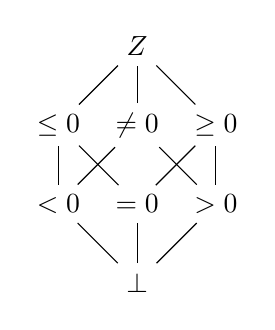
\begin{tikzpicture}
    \node [] (0) at (0, 0) {$\bot$};

    \node [] (1) at (-1, 1) {$< 0$};
    \draw (0) to (1);
    \node [] (2) at (0, 1) {$=0$};
    \draw (0) to (2);
    \node [] (3) at (+1, 1) {$> 0$};
    \draw (0) to (3);
    
    \node [] (4) at (-1, 2) {$\leq 0$};
    \draw (1) to (4);
    \draw (2) to (4);
    \node [] (5) at (0, 2) {$\neq 0$};
    \draw (1) to (5);
    \draw (3) to (5);
    \node [] (6) at (+1, 2) {$\geq 0$};
    \draw (2) to (6);
    \draw (3) to (6);
    
    \node [] (7) at (0, 3) {$\mathbb{Z}$};
    \draw (6) to (7);
    \draw (5) to (7);
    \draw (4) to (7);
  \end{tikzpicture}
  \end{center}

  Then, there is a Galois insertion from $Sign$ to $\pow{\mathbb{Z}}$ defined as:
  $$\gamma(A) = \begin{cases}
    \{ x \mid x \;op\; 0 \} & \text{if } A = op\;0 \\
    \mathbb{Z}              & \text{if } A = \mathbb{Z} \\
    \emptyset & \text{otherwise}
  \end{cases}$$
  $$\alpha(C) = \begin{cases}
    \bot & \text{if } C = \emptyset \\
    op \; 0 & \text{if } C \subseteq \{ x \mid x \; op \; 0 \}
        \mand op \in \{<, >, =, \leq, \geq, \neq \} \\
    \mathbb{Z} & \text{otherwise}
  \end{cases}$$
\end{example}

The fundamental goal of abstract interpretation is to provide an approximation 
of the non-computable aspects of program semantics. The core concept is captured 
by the definition of soundness:

\begin{definition}[Soundness]
  Given an abstract domain $A$, an abstract function $f^\# : A \to A$ is a 
  sound approximation of a concrete function $f : \pow{\states} \to 
  \pow{\states}$ if
  $$\alpha(f(P)) \leq f^\#(\alpha(P))$$
\end{definition}

Hence, the goal of abstract interpretation is to construct a sound 
over-approximation of the program semantics that is computable (efficiently).

\begin{example}
  We can use the sign domain to construct a sound approximation of the
  multiplication operation: 
  \begin{table}[h!]
    \centering
    \begin{tabular}{|c|c|c|c|c|c|c|c|c|}
      \hline
      $\times^\#$ & $\bot$ & $< 0$ & $> 0$ & $= 0$ & $\le 0$ & $\ne 0$ & $\ge 0$ 
                  & $\mathbb{Z}$ \\
      \hline
      $\bot$ & $\bot$ & $\bot$ & $\bot$ & $\bot$ & $\bot$ & $\bot$ & $\bot$ 
             & $\bot$ \\
      \hline
      $< 0$ & $\bot$ & $> 0$ & $< 0$ & $= 0$ & $< 0$ & $\ne 0$ & $\le 0$ 
            & $\mathbb{Z}$ \\
      \hline
      $> 0$ & $\bot$ & $< 0$ & $> 0$ & $= 0$ & $\le 0$ & $\ne 0$ & $\ge 0$ 
            & $\mathbb{Z}$ \\
      \hline
      $= 0$ & $\bot$ & $= 0$ & $= 0$ & $= 0$ & $= 0$ & $= 0$ & $= 0$ & $= 0$ \\
      \hline
      $\le 0$ & $\bot$ & $< 0$ & $\le 0$ & $= 0$ & $\le 0$ & $\ne 0$ & $\le 0$ 
              & $\mathbb{Z}$ \\
      \hline
      $\ne 0$ & $\bot$ & $\ne 0$ & $\ne 0$ & $= 0$ & $\ne 0$ & $\ne 0$ 
              & $\ne 0$ & $\mathbb{Z}$ \\
      \hline
      $\ge 0$ & $\bot$ & $\le 0$ & $\ge 0$ & $= 0$ & $\le 0$ & $\ne 0$ 
              & $\ge 0$ & $\mathbb{Z}$ \\
      \hline
      $\mathbb{Z}$ & $\bot$ & $\mathbb{Z}$ & $\mathbb{Z}$ & $= 0$ 
                   & $\mathbb{Z}$ & $\mathbb{Z}$ & $\mathbb{Z}$ & $\mathbb{Z}$ \\
      \hline
    \end{tabular}
    \caption{Multiplication table for $Sign$ domain}
  \end{table}
\end{example}
\chapter{The abstract Hoare logic framework}


In this chapter, we will develop the minimal theory of \textit{Abstract Hoare
Logic}. We will formalize the extensible language $\lang$, a minimal imperative
programming language that is parametric on a set of basic commands to permit
the definition of arbitrary program features, such as pointers, objects, etc.
We will define the semantics of the language, provide the standard definition
of Hoare triples, and introduce the concept of abstract inductive semantics; a
modular approach to express the strongest postcondition of a program, where the
assertion language is a complete lattice. Additionally, we will present a sound
and complete proof system to reason about these properties.

\section{The $\lang$ programming language}

\subsection{Syntax}

The $\lang$ language is inspired by Dijkstra's guarded command languages
\cite{Dijkstra74} with the goal of being as general as possible by being
parametric on a set of \textit{basic commands}. The $\lang$ language is general
enough to describe any imperative non-deterministic programming language.

\begin{definition}[$\lang$ language syntax]
  Given a set $BCmd$ of basic commands, the set on valid $\lang$ programs is 
  defined by the following inductive definition:

  \begin{align*}
    b \in BCmd \\
    \lang \ni C, C_1, C_2 \; & \cceq \sskip        & \text{Skip}\\
                             & \smid b             & \text{Basic command}\\
                             & \smid C_1 \fcmp C_2 & \text{Program composition}\\
                             & \smid C_1 + C_2     & \text{Non deterministic choice}\\
                             & \smid C^\fix        & \text{Iteration}\\
  \end{align*}

  \begin{example} \label{exmp:base-commands-syntax}
    Usually the set of basic commands contains a command to perform tests $e ?$
    discarding executions that do not satisfy the predicate $e$, and $x \ass v$
    to assign the value $v$ to the variable $x$.
  \end{example}
\end{definition}


\subsection{Semantics}

Fixed a set $\states$ of states (usually a collection of associations between
variables names and values) and a family of partial functions $\bsem{\cdot} :
BCmd \to \states \topartial \states$ we can define the denotational semantics
of programs in $\lang$. The \textit{collecting semantics} is defined as a function
$\sem{\cdot} : \lang \to \pow{\states} \to \pow{\states}$ that associates a
program $C$ and a set of initial states to the set of states reached after
executing the program $C$ from the initial states, this is also know as the
predicate transformer semantics \cite{Dijkstra74}.

\begin{definition}[Denotational semantics]
  \label{def:deno}
  Given a set $\states$ of states and a family of partial functions
  $\bsem{\cdot} : BCmd \to \states \topartial \states$ the denotational
  semantics is defined as follows:

  \begin{align*}
      \sem{\cdot}         & \;\;:\; \lang \to \pow{\states} \to \pow{\states} \\
      \sem{\sskip}        &\defeq id \\
      \sem{b}             &\defeq \lambda P . \{ \bsem{b}(p)\downarrow \; \mid 
        p \in P \} \\
      \sem{C_1 \fcmp C_2} &\defeq \sem{C_2} \circ \sem{C_1} \\
      \sem{C_1 + C_2}     &\defeq \lambda P . \sem{C_1} P \cup \sem{C_2} P \\
      \sem{C^\fix}        &\defeq \lambda P . \lfp(\lambda P'. P \cup \sem{C} P')
  \end{align*}

  \begin{example}
    We can define the semantics of the basic commands introduced in 
    \ref{exmp:base-commands-syntax} as:
    $$\bsem{e ?}(\sigma) \defeq \begin{cases}
      \; \sigma & \sigma \models e \\
      \; \uparrow & otherwise
    \end{cases}$$

    Where $\sigma \models e$ means that the state $\sigma$ satisfies the 
    predicate $e$ and $\uparrow$ is denoting that the function is diverging.

    $$\bsem{x \ass e}(\sigma) \defeq \sigma[x/eval(e, \sigma)]$$
    Where $eval$ is some evaluate function for the expressions on the left-hand
    side of assignments and then is substitute in place of $x$ in the 
    state $\sigma$.
  \end{example}

  \begin{theorem}[Monotonicity]
    \label{thm:sem-mono}
    $\forall \; C \in \lang$ $\sem{C}$ is well-defined and monotone.
  \end{theorem}
  \begin{proof}
    We want to prove that $\forall P, Q \in \pow{\states}$ and $C \in \lang$
    $$P \subseteq Q \implies \sem{C}(P) \subseteq \sem{C}(Q)$$
    By structural induction on $C$:
    \begin{itemize}
      \item $\sskip$:
        \begin{align*}
          \sem{\sskip}(P) 
            &= P
            & \text{[By definition of $\sem{\sskip}$]}\\
            &\subseteq Q \\
            &= \sem{\sskip}(Q) 
            & \text{[By definition of $\sem{\sskip}$]}\\
        \end{align*}

      \item $b$:
        \begin{align*}
          \sem{b}(P) 
            &= \{ \bsem{b}(x)\downarrow \; \mid x \in P \} 
            & \text{[By definition of $\sem{b}$]}\\
            &\subseteq \{ \bsem{b}(x)\downarrow \; \mid x \in Q \} 
            & \text{[Since $P \subseteq Q$]}\\
            &= \sem{b}(Q) 
            & \text{[By definition of $\sem{b}$]}\\
        \end{align*}

      \item $C_1 \fcmp C_2$:

        By inductive hypothesis $\sem{C_1}$ is monotone hence
        $\sem{C_1}(P) \subseteq \sem{C_2}(Q)$

        \begin{align*}
          \sem{C_1 \fcmp C_2}(P) 
            &= \sem{C_2}(\sem{C_1}(P))
            &\text{[By definition of $\sem{C_1 \fcmp C_2}$]}\\
            &\subseteq \sem{C_2}(\sem{C_1}(Q))
            &\text{[By inductive hypothesis on $\sem{C_2}$]} \\
        \end{align*}
    
      \item $C_1 + C_2$:
        \begin{align*}
          \sem{C_1 + C_2}(P) 
            &= \sem{C_1}(P) \cup \sem{C_2}(P)
            &\text{[By definition of $\sem{C_1 + C_2}$]}\\
            &\subseteq \sem{C_1}(Q) \cup \sem{C_2}(P)
            &\text{[By inductive hypothesis on $\sem{C_1}$]} \\
            &\subseteq \sem{C_1}(Q) \cup \sem{C_2}(Q)
            &\text{[By inductive hypothesis on $\sem{C_2}$]} \\
            &= \sem{C_1 + C_2}(Q) 
            &\text{[By definition of $\sem{C_1 + C_2}$]}\\
        \end{align*}
      
      \item $C^\fix$:

        \begin{align*}
          \sem{C^\fix}(P) 
            &= \lfp(\lambda P'. P \cup \sem{C}(P'))
            &\text{[By definition of $\sem{C^\fix}$]}\\
            &\subseteq \lfp(\lambda P'. Q \cup \sem{C}(P'))
            &\text{[By theorem \ref{thm:lfp-mono}]}\\
            &= \sem{C^\fix}(Q) 
            &\text{[By definition of $\sem{C^\fix}$]}\\
        \end{align*}
        
        Clearly all the $\lfp$ are well-defined since by inductive hypothesis
        $\sem{C}$ is monotone and $\pow{\states}$ is a complete from 
        \ref{thm:knaster} the least-fixpoint exists.
    \end{itemize}

  \end{proof}

  \begin{observation}
    As observed in \cite{Fischer79} when the set of basic commands contains a 
    command to discard executions we can define the usual deterministic control 
    flow commands as syntactic sugar.

    $$\bm{if} \; b \; \bm{then} \; C_1 \; \bm{else} \; C_2 \defeq (b ? \fcmp C_1) 
    + (\neg b ? \fcmp C_2)$$
    $$\bm{while} \; b \; \bm{do} \; C \defeq (b? \fcmp C)^\fix \fcmp \neg b ?$$
  \end{observation}

  \begin{observation}
    Regular languages of Kleene algebras \cite{Kozen97} usually provide an
    iteration command usually denoted $C^\star$ whose semantics is
    $\sem{C^\star}(P) \defeq \bigcup_{n \in \nat} \sem{C}^n(P)$. This is
    equivalent to $C^\fix$, the reasoning on why a fixpoint formulation was
    chosen will become clear in \ref{obs:abstract-fix}.
  \end{observation}

  \begin{example}
    Let $C \defeq (x \leq 10? \fcmp x := x + 1)^\fix + (x := 55)$ and 
    $P = \{ x = 1 \}$ then we can compute $\sem{C}(P)$ as:
    \begin{align*}
      \sem{C}(P)
        &= \sem{(x \leq 10? \fcmp x := x +1)^\fix}(P) \cup \sem{x := 55}(P) \\
        &= \lfp(\lambda P' . P \cup \sem{x \leq 10? \fcmp x := x + 1}(P'))
          \cup \{x = 55\} \\
        &= \{ x \in \{1, ..., 10\} \} \cup \{x = 55\} \\
        &= \{ x \in \{1, ..., 10, 55\} \}
    \end{align*}
  \end{example}

\end{definition}

\section{Abstract inductive semantics}

From the theory of abstract interpretation we know that the definition of the
denotational semantics can be modified to work on any complete lattice as long
as we provide suitable function for the basic commands. The rationale
behind is the same as in the denotational semantics but instead of representing
collections of states with $\pow{\states}$ now they are represented in an
arbitrary complete lattice.

\begin{definition}[Abstract inductive semantics]

  \label{def:abstract-inductive-semantics}
  Given a complete lattice $A$ and a family of monotone functions $\bsem{\cdot}^A : 
  BCmd \to A \to A$ the abstract inductive semantics is defined inductively as 
  follows:

  \begin{align*}
      \asem{\cdot}         & \;\;:\; \lang \to A \to A \\
      \asem{\sskip}         &\defeq id \\
      \asem{b}             &\defeq \bsem{b}^A \\
      \asem{C_1 \fcmp C_2} &\defeq \asem{C_2} \circ \asem{C_1} \\
      \asem{C_1 + C_2}     &\defeq \lambda P . \asem{C_1} P \join_A \asem{C_2} P \\
      \asem{C^\fix}        &\defeq \lambda P . \lfp(\lambda P'. P \join_A \asem{C} P')
  \end{align*}
\end{definition}


When designing abstract interpreters to perform abstract interpretation,
iterative commands are usually not expressed directly as fixpoints but by
some over-approximation, as is the case for the $C^\fix$ command. This is
necessary since the goal of the abstract interpreter is to be executed and, in
general, if the lattice on which the interpretation executed run has infinite
ascending chains, it's computation can diverge. In our case, the termination
requirement isn't necessary since we are not interested in computing the abstract
inductive semantics but using it as a reference on which the definition of
abstract Hoare logic is dependent.


As we did for the concrete collecting semantics, we need to prove that the
semantics is well-defined. In general, if we drop the requirement for $A$
to be a complete lattice or for $\bsem{b}$ to be monotone, the least fixpoint
could be undefined.

\begin{theorem}[Monotonicity]
  \label{thm:asem-mono} 
  $\forall \; C \in \lang$ $\asem{C}$ is well-defined and monotone.
\end{theorem}
\begin{proof}
  We want to prove that $\forall P, Q \in A$ and $C \in \lang$
  $$P \leq_A Q \implies \asem{C}(P) \leq_A \asem{C}(Q)$$
  By structural induction on $C$:
  \begin{itemize}
    \item $\sskip$:
      \begin{align*}
        \asem{\sskip}(P) 
          &= P 
          & \text{[By definition of $\asem{\sskip}$]}\\
          &\leq Q \\
          &= \asem{\sskip}(Q) 
          & \text{[By definition of $\asem{\sskip}$]}\\
      \end{align*}

    \item $b$:
      \begin{align*}
        \asem{b}(P) 
          &= \bsem{b}^A(P)
          & \text{[By definition of $\asem{b}$]}\\
          &\leq \bsem{b}^A(Q)
          & \text{[By definition]}\\
          &= \asem{b}(Q) 
          & \text{[By definition of $\asem{b}$]}\\
      \end{align*}

    \item $C_1 \fcmp C_2$:

      By inductive hypothesis $\asem{C_1}$ is monotone hence
      $\asem{C_1}(P) \leq_A \asem{C_1}(Q)$

      \begin{align*}
        \asem{C_1 \fcmp C_2}(P) 
          &= \asem{C_2}(\asem{C_1}(P))
          &\text{[By definition of $\asem{C_1 \fcmp C_2}$]}\\
          &\leq_A \asem{C_2}(\asem{C_1}(Q))
          &\text{[By inductive hypothesis on $\asem{C_2}$]} \\
      \end{align*}
  
    \item $C_1 + C_2$:
      \begin{align*}
        \asem{C_1 + C_2}(P) 
          &= \asem{C_1}(P) \join_A \asem{C_2}(P)
          &\text{[By definition of $\asem{C_1 + C_2}$]}\\
          &\leq_A \asem{C_1}(Q) \join_A \asem{C_2}(P)
          &\text{[By inductive hypothesis on $\asem{C_1}$]} \\
          &\leq_A \asem{C_1}(Q) \join_A \asem{C_2}(Q)
          &\text{[By inductive hypothesis on $\asem{C_2}$]} \\
          &= \asem{C_1 + C_2}(Q) 
          &\text{[By definition of $\asem{C_1 + C_2}$]}\\
      \end{align*}
    
    \item $C^\fix$:

      \begin{align*}
        \asem{C^\fix}(P) 
          &= \lfp(\lambda P'. P \join_A \asem{C}(P'))
          &\text{[By definition of $\asem{C^\fix}$]}\\
          &\leq_A \lfp(\lambda P'. Q \join_A \asem{C}(P'))
          &\text{[By theorem \ref{thm:lfp-mono}]}\\
          &= \asem{C^\fix}(Q) 
          &\text{[By definition of $\asem{C^\fix}$]}\\
      \end{align*}
  \end{itemize}


  Clearly all the $\lfp$ are well-defined since by inductive hypothesis
  $\sem{C}$ is monotone and $A$ is a complete from 
  \ref{thm:knaster} the least-fixpoint exists.
\end{proof}

From now on we will refer to the complete lattice $A$ used to define the abstract
inductive semantics as \textit{domain} borrowing the terminology from abstract
interpretation.

\begin{observation}
  \label{obs:post}
  When picking as a domain the lattice $\pow{\states}$ and as basic commands
  $\bsem{b}^{\pow{\states}}(P) = \{ \bsem{b}(\sigma)\downarrow \; \mid \sigma 
  \in P \}$ we will obtain the denotational semantics from the 
  abstract inductive semantics, that is: $\forall \; C \in \lang$ $\forall P \in 
  \pow{\states}$ 
  $$\asem[\pow{\states}]{C}(P) = \sem{C}(P)$$
  This can be easily checked by comparing the two definitions.
\end{observation}

From this observation, we can see that theorem \ref{thm:sem-mono} is just an
instance of theorem \ref{thm:asem-mono} since $\pow{\states}$ is a
complete lattice and the semantics of the basic commands is monotone by
construction.

\subsection{Connection with Abstract Interpretation}

As stated above, the definition of abstract inductive semantics is closely
related to the one of abstract semantics \cite{Cousot77}. In particular, the 
definition of abstract inductive semantics, when the semantics of the basic
commands is sound, is equivalent to an abstract semantics.

\begin{theorem}[Abstract interpretation instance]
  \label{thm:sound-ai}
  If $A$ is an abstract domain and $\bsem{\cdot}^A$ is a sound 
  over-approximation of $\bsem{\cdot}$, then $\asem{\cdot}$ is a sound 
  over-approximation of $\sem{\cdot}$.
\end{theorem}
\begin{proof}
  We prove $\alpha(\sem{C}(P)) \leq \asem{C}(\alpha(P))$ by structural
  induction on $C$:

  \begin{itemize}
    \item $\sskip$:
      \begin{align*}
        \alpha(\sem{\sskip}(P))
          &= \alpha(P)
          & \text{[By definition of $\sem{\sskip}$]}\\
          &= \asem{\sskip}(\alpha(P)) 
          & \text{[By definition of $\asem{\sskip}$]}\\
      \end{align*}

    \item $b$:
      \begin{align*}
        \alpha(\sem{b}(P))
          &= \bsem{b}(P)
          & \text{[By definition of $\sem{b}$]}\\
          &\leq \bsem{b}^A(\alpha(P))
          & \text{[By definition]}\\
          &= \asem{b}(\alpha(P)) 
          & \text{[By definition of $\asem{b}$]}\\
      \end{align*}

    \item $C_1 \fcmp C_2$:

      \begin{align*}
        \alpha(\sem{C_1 \fcmp C_2}(P))
          &= \alpha(\sem{C_2}(\sem{C_1}(P)))
          &\text{[By definition of $\sem{C_1 \fcmp C_2}$]}\\
          &\leq \asem{C_2}(\alpha(\sem{C_1}(P)))
          &\text{[By inductive hypothesis on $C_2$]}\\
          &\leq \asem{C_2}(\asem{C_1}(\alpha(P)))
          &\text{[By inductive hypothesis on $C_1$} \\
          && \text{and $\asem{C_2}$ monotone]}\\
          &= \asem{C_1 \fcmp C_2}(\alpha(P))
          &\text{[By definition of $\asem{C_1 \fcmp C_2}$]}\\
      \end{align*}
  
    \item $C_1 + C_2$:
      \begin{align*}
        \alpha(\sem{C_1 + C_2}(P))
          &= \alpha(\sem{C_1}(P) \cup \sem{C_2}(P))
          &\text{[By definition of $\sem{C_1 + C_2}$]}\\
          &\leq \alpha(\sem{C_1}(P)) \join \alpha(\asem{C_2}(P)) \\
          &\leq \asem{C_1}(\alpha(P)) \join \asem{C_2}(\alpha(P))
          &\text{[By inductive hypothesis on $C_1$} \\
          && \text{and $C_2$]} \\
          &= \asem{C_1 + C_2}(\alpha(P))
          &\text{[By definition of $\asem{C_1 + C_2}$]}\\
      \end{align*}
    
    \item $C^\fix$:

      \begin{align*}
        \alpha(\sem{C^\fix}(P) )
          &= \alpha(\lfp(\lambda P'. P \cup \sem{C}(P')))
          &\text{[By definition of $\sem{C^\fix}$]}\\
          &= \alpha(\bigcup_{n \in \mathbb{N}}{\sem{C}^n(P)}) \\
          &\leq \bigvee_{n \in \mathbb{N}}{\alpha(\sem{C}^n(P))}) \\
          &\leq \bigvee_{n \in \mathbb{N}}{(\asem{C})^n(\alpha(P))}
          &\text{[By inductive hypothesis on $C$]}\\
          &\leq \lfp(\lambda P'. \alpha(P) \join \asem{C}(P')) \\
          &= \asem{C^\fix}(\alpha(P)) 
          &\text{[By definition of $\asem{C^\fix}$]}\\
      \end{align*}
  \end{itemize}
\end{proof}

This connection also allows us to obtain abstract inductive semantics through 
Galois insertions.

\begin{definition}[Abstract Inductive Semantics by Galois Insertion]
  \label{def:aisgi}
  Let $\langle C, \sqsubseteq \rangle \galoiS{\alpha}{\gamma} \langle A, \leq
  \rangle$ be a Galois insertion, and let $\asem[C]{C}$ be some abstract
  inductive semantics defined on $C$. Then, the abstract inductive semantics
  defined on $A$ with $\bsem{b}^A \defeq \alpha \circ \bsem{c}^C \circ \gamma$
  is the abstract inductive semantics obtained by the Galois insertion between
  $C$ and $A$.
\end{definition}

The abstract inductive semantics obtained by Galois insertion between 
$\pow{\states}$ and any domain $A$ corresponds to the best abstract inductive 
interpreter on $A$.

\begin{observation}
  \label{obs:abstract-fix}
  There are some domains where $\exists \; C \in \lang$ such that
  $\bigvee_{n \in \nat} (\asem{C})^n(P) \neq \lfp(\lambda P'. P \join_A
  \asem{C}(P'))$.
\end{observation}
\begin{example}
  Let $C \defeq (x > 1? \fcmp ((even(x) ? \fcmp X := x + 3) +
  (\neg even(x)? \fcmp x := x - 2))^\fix$ when performing the computation on
  the interval domain, if we compute $C$ using the infinitary join:
  \begin{align*}
    \asem{C}([5, 5])
      &= \bigvee_{n \in \mathbb{N}} (\asem{x > 1? \fcmp ((even(x) ? \fcmp x :=
        x + 3) + (\neg even(x)? \fcmp x := x - 2))})^n([5, 5]) \\
      &= [5, 5] \join [3, 3] \join [1, 1] \join \bot \join \bot ... \\
      &= [1, 5]
  \end{align*}

  The difference is caused by the fact that when we are computing the infinite 
  join, all the joins happen after executing the semantics of the loop body.
  
\end{example}
\section{Abstract Hoare Logic}
\label{chp:intro-ahorare}

\subsection{Hoare logic}
Hoare logic  \cite{Hoare69, Floyd93} was one of the first method designed for 
the verification of programs, It's core concept is that of partial correctness 
assertions. A Hoare triple is a formula $\htriple{P}{C}{Q}$ where $P$ and $Q$ are 
assertions on the initial and final states of a program $C$, respectively. 
These assertions are partial in the sense that $Q$ is meaningful only when the 
execution of $C$ on $P$ terminates.

Hoare logic is designed as a proof system, where the syntax 
$\vdash \htriple{P}{C}{Q}$ indicates that the triple 
$\htriple{P}{C}{Q}$ is proved by applying the rules of the proof system.

The original formulation of Hoare logic was given for an imperative language 
with deterministic constructs, but it can be easily defined for our language 
$\lang$ following the work in \cite{Moller21}.

\begin{definition}[Hoare triple]
  \label{def:hoare}
  Fixed the semantics of the basic commands, an Hoare triple denoted by 
  $\htriple{P}{C}{Q}$, is valid if and only if $\sem{C}(P) \subseteq Q$.

  $$\models \htriple{P}{C}{Q} \iff \sem{C}(P) \subseteq Q$$
\end{definition}

We will use the syntax $\models \htriple{P}{C}{Q}$ to refer to valid triples,
$\not \models \htriple{P}{C}{Q}$ to refer to invalid triples, and
$\htriple{P}{C}{Q}$ when we are not asserting the validity or invalidity of a
triple.

\begin{example}[Hoare triples]
  \label{exmp:hlogic}
We have that $\htriple{x \in [1, 2]}{x := x + 1}{x \in [2, 3]}$, is a
valid triple since from any state in which either $x = 1$ or $x = 2$,
incrementing by one the value of $x$ leads to states in which $x$ is either $2$
or $3$. Specifically, starting from $x = 1$ leads us to $x = 2$ and starting
from $x = 2$ leads us to $x = 3$.

Since the conclusion of Hoare triples must contain all the final states, the
triple $\htriple{P}{C}{\top}$ is always valid since $\top$ contains all the
possible states.

An example of an invalid triple is $\htriple{x \in [1, 2]}{x := x
+ 1}{x \in [1, 2]}$ since the state $x = 2$ satisfies the precondition and
executing the program on it results in the state $x = 3$, which does not satisfy
$x \in [1, 2]$.

Since Hoare logic is concerned only with termination, when the program is
non-terminating, we can prove any property. For example, $\htriple{x
\in [0, 10]}{(x \leq 20? \fcmp x := x - 1)^\fix \fcmp x \geq 20?}{Q}$ is always
a valid triple since the program is non-terminating for any $x \in [0, 10]$. 
The set of reachable states is empty, thus the postcondition is vacuously true.

This is the reason why Hoare logic is called a partial correctness logic,
where partial means that it can prove the adherence of a program to
some specification only when it is terminating. The termination of the program
must be proved by resorting to some alternative method.
\end{example}

\begin{definition}[Hoare logic]$\;$ \\
  \label{def:hoaretules}
  The rules of Hoare logic are defined as follows:
  \begin{prooftree}
    \AxiomC{$ $}
    \RightLabel{$(\sskip)$}
    \UnaryInfC{$\vdash \htriple{P}{\sskip}{P}$}
  \end{prooftree}

  % Rule for a basic command
  \begin{prooftree}
    \AxiomC{$ $}
    \RightLabel{$(base)$}
    \UnaryInfC{$\vdash \htriple{P}{b}{\bsem{b}(P)}$}
  \end{prooftree}

  % Rule for sequential composition
  \begin{prooftree}
    \AxiomC{$\vdash \htriple{P}{C_1}{Q}$}
    \AxiomC{$\vdash \htriple{Q}{C_2}{R}$}
    \RightLabel{$(seq)$}
    \BinaryInfC{$\vdash \htriple{P}{C_1 \fcmp C_2}{R}$}
  \end{prooftree}

  % Rule for nondeterministic choice
  \begin{prooftree}
    \AxiomC{$\vdash \htriple{P}{C_1}{Q}$}
    \AxiomC{$\vdash \htriple{P}{C_2}{Q}$}
    \RightLabel{$(disj)$}
    \BinaryInfC{$\vdash \htriple{P}{C_1 + C_2}{Q}$}
  \end{prooftree}

  \begin{prooftree}
    \AxiomC{$\vdash \htriple{P}{C}{P}$}
    \RightLabel{$(iterate)$}
    \UnaryInfC{$\vdash \htriple{P}{C^\fix}{P}$}
  \end{prooftree}

  % Rule for strengthening the precondition and weakening the postcondition
  \begin{prooftree}
    \AxiomC{$P \subseteq P'$}
    \AxiomC{$\vdash \htriple{P'}{C}{Q'}$}
    \AxiomC{$Q' \subseteq Q$}
    \RightLabel{$(consequence)$}
    \TrinaryInfC{$\vdash \htriple{P}{C}{Q}$}
  \end{prooftree}
\end{definition}

The proof system described in Definition \ref{def:hoaretules} is logically
sound, meaning that all it's provable triples are valid with respect to
definition \ref{def:hoare}.

\begin{theorem}[Soundness]
  $$\vdash \htriple{P}{C}{Q} \implies \models \htriple{P}{C}{Q}$$
\end{theorem}

As observed by Cook \cite{Cook78}, the reverse implication is not true, in 
general, as a consequence of Gödel's incompleteness theorem. For this reason, 
Cook developed the concept of relative completeness, in which all the instances 
of $\subseteq$ are provided by an oracle, proving that the incompleteness of the 
proof system is only caused by the incompleteness of the assertion language.

\begin{theorem}[Relative completeness]
  \label{thm:hlogic-complete}
  $$\models \htriple{P}{C}{Q} \implies \vdash \htriple{P}{C}{Q}$$
\end{theorem}

\subsection{Abstracting Hoare logic}
The idea of designing a Hoare-like logic to reason about properties of programs
expressible within the theory of lattices using concepts from abstract
interpretation is not new. In fact, \cite{Cousot12} already proposed a
framework to perform this kind of reasoning. However, the validity of the
triples in \cite{Cousot12} dependends on the standard definition of Hoare
triples, and the proof system is incomplete if we ignore the rule to embed
standard Hoare triples in the abstract ones.

Our approach will be different. In particular, the meaning of abstract Hoare 
triples will be dependent on the abstract inductive semantics, and we will 
provide a sound and (relatively) complete without resorting to embedd Hoare 
logic in it's proof system as \cite{Cousot12}.

\begin{definition}[Abstract Hoare triple]
  \label{def:aht}
  Given an abstract inductive semantics $\asem{\cdot}$ on the complete lattice
  $A$, the abstract Hoare triple written $\atriple{P}{C}{Q}$ is valid if
  and only if $\asem{C}(P) \leq_A Q$.

  $$\models \atriple{P}{C}{Q} \iff \asem{C}(P) \leq_A Q$$
\end{definition}

The definition is equivalent to the definition \ref{def:hoare} 
but here the abstract inductive semantics is used to provide the strongest 
postcondition of programs.

In Abstract Hoare logic some of the examples shown in example \ref{exmp:hlogic} 
still hold, in particular we have that:
\begin{example}
  $$\models \atriple{P}{C}{\top}$$
\end{example}
\begin{proof}
  \begin{align*}
    \models \atriple{P}{C}{\top}
      & \iff \asem{C}(P) \leq \top & \text{By definition of $\atriple{\cdot}{\cdot}{\cdot}$} \\
  \end{align*}

  And since $\top$ is the top element of $A$ $\top \geq \asem{C}(P)$
\end{proof}

\subsubsection{2.3.3 Proof system}
As per Hoare logic we will provide a sound and relatively complete (in the sense
of \cite{Cook78}) proof system to derive abstract Hoare triples in a 
compositional fashion.

\begin{definition}[Abstract Hoare rules]$\;$\\
  \label{def:ahtrules}
  % Rule for the identity command
  \begin{prooftree}
    \AxiomC{$ $}
    \RightLabel{$(\sskip)$}
    \UnaryInfC{$\vdash \atriple{P}{\sskip}{P}$}
  \end{prooftree}

  % Rule for a basic command
  \begin{prooftree}
    \AxiomC{$ $}
    \RightLabel{$(b)$}
    \UnaryInfC{$\vdash \atriple{P}{b}{\bsem{b}^A(P)}$}
  \end{prooftree}

  % Rule for sequential composition
  \begin{prooftree}
    \AxiomC{$\vdash \atriple{P}{C_1}{Q}$}
    \AxiomC{$\vdash \atriple{Q}{C_2}{R}$}
    \RightLabel{$(\mathbb{\fcmp})$}
    \BinaryInfC{$\vdash \atriple{P}{C_1 \fcmp C_2}{R}$}
  \end{prooftree}

  % Rule for nondeterministic choice
  \begin{prooftree}
    \AxiomC{$\vdash \atriple{P}{C_1}{Q}$}
    \AxiomC{$\vdash \atriple{P}{C_2}{Q}$}
    \RightLabel{$(+)$}
    \BinaryInfC{$\vdash \atriple{P}{C_1 + C_2}{Q}$}
  \end{prooftree}

  % Rule for iteration (Kleene star)
  \begin{prooftree}
    \AxiomC{$\vdash \atriple{P}{C}{P}$}
    \RightLabel{$(\fix)$}
    \UnaryInfC{$\vdash \atriple{P}{C^\fix}{P}$}
  \end{prooftree}

  % Rule for strengthening the precondition and weakening the postcondition
  \begin{prooftree}
    \AxiomC{$P \leq P'$}
    \AxiomC{$\vdash \atriple{P'}{C}{Q'}$}
    \AxiomC{$Q' \leq Q$}
    \RightLabel{$(\leq)$}
    \TrinaryInfC{$\vdash \atriple{P}{C}{Q}$}
  \end{prooftree}
\end{definition}

The rules can be summarized as:
\begin{itemize}
  \item The identity command does not change the state, so if $P$ holds before,
    it will hold after the execution.

  \item For a basic command $b$, if $P$ holds before the execution, then 
    $\bsem{b}^A(P)$ holds after the execution.

  \item If executing $C_1$ from state $P$ leads to state $Q$, and executing
    $C_2$ from state $Q$ leads to state $R$, then executing $C_1$ followed by
    $C_2$ from state $P$ leads to state $R$.

  \item If executing either $C_1$ or $C_2$ from state $P$ leads to state $Q$,
    then executing the nondeterministic choice $C_1 + C_2$ from state $P$ also
    leads to state $Q$.

  \item If executing command $C$ from state $P$ leads back to state $P$, then
    executing $C$ repeatedly (zero or more times) from state $P$ also leads
    back to state $P$.

  \item If $P$ is stronger than $P'$ and $Q'$ is stronger than $Q$, then we can
    derive $\atriple{P}{C}{Q}$ from $\atriple{P'}{C}{Q'}$.
\end{itemize}

The proofsystem is nonother than definition \ref{def:hoaretules},
where the assertion are replaced by elements of the complete lattice $A$.

Note that we denote Abstract Hoare Triples as defined in defintion \ref{def:aht}
with the notation $\atriple{P}{C}{Q}$ while we denote the triples obtained
with the inference rules of definition \ref{def:ahtrules} by $\vdash 
\atriple{P}{C}{Q}$.

The proofsystem for Abstract Hoare logic is sound, as the original Hoare logic.

\begin{theorem}[Soundness]
  \label{thm:atriple-sound}
  $$\vdash \atriple{P}{C}{Q} \implies \models \atriple{P}{C}{Q}$$
\end{theorem}
\begin{proof}
  By structural induction on the last rule applied in the derivation of
  $\vdash \atriple{P}{C}{Q}$:
  \begin{itemize}

    \item $(\sskip)$:
      Then the last step in the derivation was: 
      \begin{prooftree}
        \AxiomC{$ $}
        \RightLabel{$(\sskip)$}
        \UnaryInfC{$\vdash 
          \atriple{P}{\sskip}{P}$}
      \end{prooftree}

      The triple is valid since:
      \begin{align*}
        \asem{\sskip}(P)
          &= P 
          &\text{[By definition of $\asem{\cdot}$]}
      \end{align*}

      \item $(b)$:
        Then the last step in the derivation was:
        \begin{prooftree}
          \AxiomC{$ $}
          \RightLabel{$(b)$}
          \UnaryInfC{$\vdash 
          \atriple{P}{b}{\bsem{b}^A(P)}$}
        \end{prooftree}

        The triple is valid since:
        \begin{align*}
          \asem{b}(P)
            &= \bsem{b}^A(P)
            & \text{[By definition of $\asem{\cdot}$]}
        \end{align*}

      \item $(\fcmp)$: Then the last step in the derivation was:
        \begin{prooftree}
          \AxiomC{$\vdash \atriple{P}{C_1}{Q}$}
          \AxiomC{$\vdash \atriple{Q}{C_2}{R}$}
          \RightLabel{$(\mathbb{\fcmp})$}
          \BinaryInfC{$\vdash \atriple{P}{C_1 \fcmp C_2}
            {R}$}
        \end{prooftree}
          
        By inductive hypothesis:
        $\asem{C_1}(P) \leq_A Q$ and
        $\asem{C_2}(Q) \leq_A R$.

        The triple is valid since:
        \begin{align*}
          \asem{C_1 \fcmp C_2}(P)
            &= \asem{C_2}(\asem{C_1}(P))
            &\text{[By definition of $\asem{\cdot}$]} \\
            &\leq_A \asem{C_2}(Q)
            &\text{[By monotonicity of $\asem{\cdot}$]} \\
            &\leq_A R
        \end{align*}

      \item $(+)$: Then the last step in the derivation was:
        \begin{prooftree}
          \AxiomC{$\vdash \atriple{P}{C_1}{Q}$}
          \AxiomC{$\vdash \atriple{P}{C_2}{Q}$}
          \RightLabel{$(+)$}
          \BinaryInfC{$\vdash \atriple{P}{C_1 + C_2}{Q}$}
        \end{prooftree}

        By inductive hypothesis: $\asem{C_1}(P) \leq Q$ and
        $\asem{C_2}(P) \leq Q$.

        The triple is valid since:
        \begin{align*}
          \asem{C_1 + C_2}(P)
            &= \asem{C_1}(P) \join_A \asem{C_2}(P)
            &\text{[By definition of $\asem{\cdot}$]} \\
            &\leq_A Q \join_A Q \\
            &= Q
        \end{align*}

      \item $(\fix)$:
        Then the last step in the derivation was:
        \begin{prooftree}
          \AxiomC{$\vdash \atriple{P}{C}{P}$}
          \RightLabel{$(\fix)$}
          \UnaryInfC{$\vdash \atriple{P}{C ^ \lfp}{P}$}
        \end{prooftree}

        By inductive hypothesis: $\asem{C}P \leq P$

        \begin{align*}
          \asem{C^\fix}(P)
            &= \lfp(\lambda P' \to P \join_A \asem{C}(P')) \\
        \end{align*}

        We will show that $P$ is a fixpoint of 
        $\lambda P' \to P \join_A \asem{C}(P')$.

        \begin{align*}
          (\lambda P' \to P \join_A \asem{C}(P'))(P)
            &= P \join_A \asem{C}(P)
            & \text{[since $\asem{C}(P) \leq P$]} \\
            &= P
        \end{align*}

        Hence $P$ is a fixpoint of $\lambda P' \to P \join_A \asem{C}(P')$,
        therefore it's at leas as big as the least one, $\lfp(\lambda P' \to P 
        \join_A \asem{C}(P')) \leq_A P$ thus making the triple valid.

      \item $(\leq)$: Then the last step in the derivation was:
        \begin{prooftree}
          \AxiomC{$P \leq P'$}
          \AxiomC{$\vdash \atriple{P'}{C}{Q'}$}
          \AxiomC{$Q' \leq Q$}
          \RightLabel{$(\leq)$}
          \TrinaryInfC{$\vdash \atriple{P}{C}{Q}$}
        \end{prooftree}

        By inductive hypothesis: $\asem{C}(P') \leq_A Q'$.
        
        The triple is valid since:
        \begin{align*}
          \asem{C}(P)
            & \asem{C}(P')
            & \text{[By monotonicity of $\asem{\cdot}$]}\\
            & \leq_A Q' 
            & \text{[By inductive hypothesis]} \\
            & \leq_A Q
        \end{align*}
  \end{itemize}
\end{proof}

The proof system turns out to be relatively complete aswell, in the sense that
the axioms are complete relative to what we can prove in the underlying
assertion language, that in our case is described by the complete lattice.

We will first prove a slightly weaker result, where we will show that we can
prove the strongest post-condition of every program.

\begin{theorem}[Relative $\asem{\cdot}$-completeness]
  \label{thm:post-completeness}
  $$\vdash \atriple{P}{C}{\asem{C}(P)}$$
\end{theorem}
\begin{proof}
  By structural induction on $C$:
  \begin{itemize}

    \item $\sskip$:
      By definition $\asem{\sskip}(P) = P$
      \begin{prooftree}
        \AxiomC{$ $}
        \RightLabel{$(\sskip)$}
        \UnaryInfC{$\vdash \atriple{P}{\sskip}{P}$}
      \end{prooftree}

      \item $b$:
        By definition $\asem{b}(P) = \bsem{b}^A(P)$
        \begin{prooftree}
          \AxiomC{$ $}
          \RightLabel{$(b)$}
          \UnaryInfC{$\vdash \atriple{P}{b}{\bsem{b}^A(P)}$}
        \end{prooftree}

      \item $C_1 \fcmp C_2$:
        By definition $\asem{C_1 \fcmp C_2}(P) = 
        \asem{C_2}(\asem{C_1}(P))$

        \begin{prooftree}
          \AxiomC{(Inductive hypothesis)}
          \noLine
          \UnaryInfC{$\vdash \atriple{P}{C_1}{\asem{C_1}(P)}$}
          \AxiomC{(Inductive hypothesis)}
          \noLine
          \UnaryInfC{$\vdash \atriple{\asem{C_1}(P)}{C_2}
            {\asem{C_2}(\asem{C_1}(P))}$}
          \RightLabel{$(\fcmp)$}
          \BinaryInfC{$\vdash \atriple{P}{C_1 \fcmp C_2}
            {\asem{C_2}(\asem{C_1}(P))}$}
        \end{prooftree}


      \item $C_1 + C_2$:
        By definition $\bsem{C_1 + C_2}(P) = 
        \bsem{C_1}(P) \join_A \bsem{C_2}(P)$

        \begin{prooftree}
          \AxiomC{$\pi_1$}
          \AxiomC{$\pi_2$}
          \RightLabel{$(+)$}
          \BinaryInfC{$\vdash \atriple{P}{C_1 + C_2}
            {\asem{C_1}(P) \join_A \asem{C_2}(P)}$}
        \end{prooftree}

        Where $\pi_1$:
        \begin{prooftree}
          \AxiomC{$P \leq_A P$}
          \AxiomC{(Inductive hypothesis)}
          \noLine
          \UnaryInfC{$\vdash \atriple{P}{C_1}{\asem{C_1}(P)}$}
          \AxiomC{$\asem{C_1}(P) \leq_A \asem{C_1}(P) \join_A \asem{C_2}(P)$}
          \RightLabel{$(\leq)$}
          \TrinaryInfC{$\vdash \atriple{P}{C_1}
            {\asem{C_1}(P) \join_A \asem{C_2}(P)}$}
        \end{prooftree}

        and $\pi_2$:
        \begin{prooftree}
          \AxiomC{$P \leq_A P$}
          \AxiomC{(Inductive hypothesis)}
          \noLine
          \UnaryInfC{$\vdash \atriple{P}{C_2}{\asem{C_2}(P)}$}
          \AxiomC{$\asem{C_2}(P) \leq_A \asem{C_1}(P) \join_A \asem{C_2}(P)$}
          \RightLabel{$(\leq)$}
          \TrinaryInfC{$\vdash \atriple{P}{C_2}
            {\asem{C_1}(P) \join_A \asem{C_2}(P)}$}
        \end{prooftree}

      \item $C^\fix$:
        By definition $\bsem{C^\fix}(P) = lfp(\lambda P' \to P \join_A
        \asem{C}(S')$.

        Let $K \defeq lfp(\lambda P' \to P \join_A \asem{C}(S')$
        hence $K = P \join_A \asem{C}(K)$ since it is a fixpoint, thus
        \begin{itemize}
          \item $\alpha_1$: $K \geq_A P$
          \item $\alpha_2$: $K \geq_A \asem{C}(K)$
        \end{itemize}

          \begin{prooftree}
            \AxiomC{$\alpha_1$}
            \AxiomC{$K \leq_A K$}
            \AxiomC{(Inductive hypothesis)}
            \noLine
            \UnaryInfC{$\vdash \atriple{K}{C}{\asem{C}(K)}$}
            \AxiomC{$\alpha_2$}
            \TrinaryInfC{$\vdash \atriple{K}{C}{K}$}
            \RightLabel{$(\fix)$}
            \UnaryInfC{$\vdash \atriple{K}{C^\fix}{K}$}
            \AxiomC{$K \leq_A K$}
            \RightLabel{$(\leq)$}
            \TrinaryInfC{$\vdash \atriple{P}{C^\fix}{K}$}
          \end{prooftree}
  \end{itemize}
\end{proof}

We can now show the relative completeness, by applying the rule $(\leq)$ to
achieve the desired post-condition.

\begin{theorem}[Relative completeness]
  \label{thm:completeness}
  $$\models \atriple{P}{C}{Q} \implies \vdash \atriple{P}{C}{Q}$$
\end{theorem}
\begin{proof}
  By definition of $\models \atriple{P}{C}{Q} \iff Q \geq_A \asem{C}(P)$

  \begin{prooftree}
    \AxiomC{$P \leq_A P$}
    \AxiomC{(By Theorem \ref{thm:post-completeness})}
    \noLine
    \UnaryInfC{$\vdash \atriple{P}{C}{\asem{C}(P)}$}
    \AxiomC{$Q \geq_A \asem{C}(P)$}
    \RightLabel{$(\leq)$}
    \TrinaryInfC{$\vdash \atriple{P}{C}{Q}$}
  \end{prooftree}
\end{proof}
\chapter{Instantiating Abstract Hoare Logic}

In this chapter, we will demonstrate how to instantiate abstract Hoare logic to
create new proof systems. We will also illustrate that the framework of
abstract Hoare logic is sufficiently general to reason about properties that
cannot be expressed in standard Hoare logic.

\section{Hoare logic}
\label{chp:inst-hoare}

Following Observation \ref{obs:post}, the abstract inductive semantics, when 
using $(\pow{\states}, \subseteq)$ as the domain and 
$\bsem{b}^{\pow{\states}}(P) = \{ \bsem{b}(\sigma) \downarrow \; \mid \sigma 
\in P \}$ as the basic command semantics, is equivalent to the denotational 
semantics given in Definition \ref{def:deno}. As we can see from the definitions 
of Hoare Logic (Definition \ref{def:hoare}) and Abstract Hoare Logic (Definition 
\ref{def:aht}), they are equivalent. Hence, in this abstraction, Abstract Hoare 
Logic and Hoare Logic have the same formulation. Since both proof systems are 
sound and (relatively) complete, they are equivalent.
\section{Absract Interval Logic and Algebraic Hoare Logic}

\subsection{Algebraic Hoare Logic}

As explained in Section \ref{chp:intro-ahorare}, Abstract Hoare Logic was
inspired by Algebraic Hoare Logic \cite{Cousot12}. Both logics can be used to
prove properties in computer-representable abstract domains.

\begin{definition}[Algebraic Hoare triple]
  Given two Galois insertions $\langle \pow{\states}, \subseteq \rangle
  \galoiS{\alpha_1}{\gamma_1} \langle A, \leq \rangle$ and $\langle
  \pow{\states}, \subseteq \rangle \galoiS{\alpha_2}{\gamma_2} \langle B,
  \sqsubseteq \rangle$, an Algebraic Hoare triple written $\ctriple{P}{C}{Q}$ is
  valid if and only if $\htriple{\gamma_1(P)}{C}{\gamma_2(Q)}$ is valid.
  $$\models \ctriple{P}{C}{Q} \iff \models \htriple{\gamma_1(P)}{C}{\gamma_2(Q)}$$
\end{definition}

From this definition, we see that Algebraic Hoare Logic is deeply connected to
standard Hoare Logic and thus to the strongest postcondition of the program in
the concrete domain.

\begin{definition}[Algebraic Hoare logic proof system\footnote{Rules
  $(\overline{\join})$ and $(\overline{\meet})$ are missing but will be
  discussed in Section \ref{chp:join-meet-rules}}]$\;$\\
  \begin{prooftree}
    \AxiomC{$ $}
    \RightLabel{$(\overline{\bot})$}
    \UnaryInfC{$\vdash \ctriple{\bot_1}{C}{Q}$}
  \end{prooftree}

  \begin{prooftree}
    \AxiomC{$ $}
    \RightLabel{$(\overline{\top})$}
    \UnaryInfC{$\vdash \ctriple{P}{C}{\top_2}$}
  \end{prooftree}
  
  \begin{prooftree}
    \AxiomC{$\models \htriple{\gamma_1(P)}{C}{\gamma_2(Q)}$}
    \RightLabel{$(\overline{S})$}
    \UnaryInfC{$\vdash \ctriple{P}{C}{Q}$}
  \end{prooftree}
  
  \begin{prooftree}
    \AxiomC{$P \leq P'$}
    \AxiomC{$\vdash \ctriple{P'}{C}{Q'}$}
    \AxiomC{$Q' \sqsubseteq Q$}
    \RightLabel{$(\overline{\Rightarrow})$}
    \TrinaryInfC{$\vdash \ctriple{P}{C}{Q}$}
  \end{prooftree}
\end{definition}

This proof system highlights that most of the work is done by rule
$(\overline{S})$, which embeds Hoare triples in Algebraic Hoare triples. One can
easily prove that the proof system is relatively complete based on the relative
completeness of Hoare logic. In particular, only the $(\overline{S})$ rule is
actually needed since all the implications in the abstract must also hold in
the concrete.

\subsection{Abstract Interval Logic}

As shown in Definition \ref{def:aisgi}, via a Galois insertion, we can obtain a similar family of triples as those in Algebraic Hoare Logic when the abstract domains used in the pre- and post-conditions are the same.

\begin{example}[Interval logic]
  \label{exmp:int-logic}
  Applying Definition \ref{def:aisgi} to the Galois insertion on the interval
  domain defined in Example \ref{exmp:interval}, we obtain a sound and
  relatively complete logic to reason about properties of programs that are
  expressible as intervals.
\end{example}

\begin{example}[Derivation in interval logic]
  \label{exmp:int-deriv}
  Let $C \defeq ((x := 1) + (x := 3)) \fcmp (x = 2? \fcmp x := 5) + (x \neq 2?
  \fcmp x := x - 1)$

  Then the following derivation is valid:

  \begin{prooftree}
    \AxiomC{$\pi_1$}
    \AxiomC{$\pi_3$}
    \RightLabel{$(\fcmp)$}
    \BinaryInfC{$\vdash \atriple[Int]{\top}{C}{[0, 5]}$}
  \end{prooftree}

  $\pi_1$:
  \begin{prooftree}
    \AxiomC{$\top \leq \top$}
    \AxiomC{$$}
    \RightLabel{$(b)$}
    \UnaryInfC{$\vdash \atriple[Int]{\top}{x := 1}{[1, 1]}$}
    \AxiomC{$[1, 1] \leq [1, 3]$}
    \TrinaryInfC{$\vdash \atriple[Int]{\top}{x := 1}{[1, 3]}$}
    \AxiomC{$\pi_2$}
    \RightLabel{$(+)$}
    \BinaryInfC{$\vdash \atriple[Int]{\top}{(x := 1) + (x := 3)}{[1, 3]}$}
  \end{prooftree}

  $\pi_2$:
  \begin{prooftree}
    \AxiomC{$\top \leq \top$}
    \AxiomC{$$}
    \RightLabel{$(b)$}
    \UnaryInfC{$\vdash \atriple[Int]{\top}{x := 3}{[3, 3]}$}
    \AxiomC{$[3, 3] \leq [1, 3]$}
    \RightLabel{$(\leq)$}
    \TrinaryInfC{$\vdash \atriple[Int]{\top}{x := 3}{[1, 3]}$}
  \end{prooftree}

  $\pi_3$:
  \begin{prooftree}
    \AxiomC{$\pi_4$}
    \AxiomC{$\pi_5$}
    \RightLabel{$(+)$}
    \BinaryInfC{$\vdash \atriple[Int]{[1, 3]}{(x = 2? \fcmp x := 5) + (x \neq 2?
      \fcmp x := x - 1)}{[0, 5]}$}
  \end{prooftree}

  $\pi_4$:
  \begin{prooftree}
    \AxiomC{$[1, 3] \leq [1, 3]$}
    \AxiomC{$$}
    \RightLabel{$(b)$}
    \UnaryInfC{$\vdash \atriple[Int]{[1, 3]}{x = 2?}{[2]}$}
    \AxiomC{$$}
    \RightLabel{$(b)$}
    \UnaryInfC{$\vdash \atriple[Int]{[2]}{x := 5}{[5]}$}
    \RightLabel{$(\fcmp)$}
    \BinaryInfC{$\vdash \atriple[Int]{[1, 3]}{x = 2? \fcmp x := 5}{[5]}$}
    \AxiomC{$[5, 5] \leq [0, 5]$}
    \RightLabel{$(\leq)$}
    \TrinaryInfC{$\vdash \atriple[Int]{[1, 3]}{x = 2? \fcmp x := 5}{[0, 5]}$}
  \end{prooftree}
  
  $\pi_5$:
  \begin{prooftree}
    \AxiomC{$[1, 3] \leq [1, 3]$}
    \AxiomC{$\pi_6$}
    \AxiomC{$[0, 2] \leq [0, 5]$}
    \TrinaryInfC{$\vdash \atriple[Int]{[1, 3]}{x \neq 2? \fcmp x := x - 1}{[0,
      5]}$}
  \end{prooftree}

  $\pi_6:$
  \begin{prooftree}
    \AxiomC{$$}
    \RightLabel{$(b)$}
    \UnaryInfC{$\vdash \atriple[Int]{[1, 3]}{x \neq 2?}{[1, 3]}$}
    \AxiomC{$$}
    \RightLabel{$(b)$}
    \UnaryInfC{$\vdash \atriple[Int]{[1, 3]}{x := x - 1}{[0, 2]}$}
    \RightLabel{$(\fcmp)$}
    \BinaryInfC{$\vdash \atriple[Int]{[1, 3]}{x \neq 2? \fcmp x := x - 1}{[0,
      2]}$}
  \end{prooftree}

  This is also the best we can derive since $\asem[Int]{C}(\top) = [0, 5]$.
\end{example}

\subsubsection{3.2.2.1 Applications}

This framework, like Algebraic Hoare Logic, can be used to specify how a static
analyzer for a given abstract domain should work. Since $\asem{\cdot}$ is the
best abstract analyzer on the abstract domain $A$ when it is defined
inductively, and since the whole proof system is in the abstract, we can check
that a derivation is indeed correct algorithmically (as long as we can check
implications and basic commands). These are usually the standard requirements
for an abstract domain to be useful. The same does not hold for Algebraic Hoare
Logic since deciding the validity of arbitrary triples would require deciding
the validity of standard Hoare logic triples, and in general, we cannot decide
implications between arbitrary properties.

\subsection{Relationship}

Clearly, Algebraic Hoare Logic can derive the same triples that are derivable
by Abstract Hoare Logic when instantiated through a Galois insertion from
$\pow{\states}$ as in Example \ref{exmp:int-logic}. From Theorem
\ref{thm:sound-ai}, $\asem{\cdot}$ is a sound overapproximation of
$\sem{\cdot}$.

\begin{theorem}
  $\vdash \atriple{P}{C}{Q} \implies \vdash \ctriple{P}{C}{Q}$
\end{theorem}
\begin{proof}
  \begin{align*}
    \vdash \atriple{P}{C}{Q}
      &\implies \asem{C}(P) \leq Q
      &\text{[From Theorem \ref{thm:atriple-sound}]} \\
      &\implies \sem{C}(\gamma(P)) \subseteq \gamma(Q)
      &\text{[From Theorem \ref{thm:sound-ai}]} \\
      &\implies \vdash \htriple{\gamma(P)}{C}{\gamma(Q)}
      &\text{[From Theorem \ref{thm:hlogic-complete}]} \\
      &\implies \vdash \ctriple{P}{C}{Q}
      &\text{[From rule $(\overline{S})$]} \\
  \end{align*}
\end{proof}

However, the converse is not true. The relative completeness of Algebraic Hoare
Logic is with respect to the best correct approximation of $\sem{\cdot}$ and not
with respect to $\asem{\cdot}$ as in Abstract Hoare Logic.

\begin{example}[Counterexample]
  From Example \ref{exmp:int-deriv}, we know that $\vdash \atriple{\top}{C}{[0, 5]}$ is
  the best Abstract Hoare triple that we can obtain, but $\sem{C}{\top} = \{0,
  2\}$. Via Theorem \ref{thm:hlogic-complete}, we can obtain
  $\vdash \htriple{\top}{C}{\{0, 2\}}$. Hence, via the $(\overline{S})$ rule, we can
  obtain $\vdash \ctriple{\top}{C}{[0, 2]}$, which is unobtainable in Abstract Hoare
  Logic.
\end{example}

This discrepancy arises because, via the $(S)$ rule in Algebraic Hoare logic,
we are able to prove the best correct approximation of any program $C$. However, the 
property of being a best correct approximation does not "compose",
meaning that the function composition of two best correct approximations is not
the best correct approximation of the composition of the functions. Since in the
abstract semantics the program composition is done in "the abstract," it's
impossible to expect to be able to obtain any possible best correct
approximation except in trivial abstract domains like the concrete
$\pow{\states}$ or the one-element lattice.

\section{Hoare logic for hyperproperties}

\renewcommand{\chi}{\mathbb{X}}

\subsection{Introduction to Hyperproperties} \label{chp:hyper}

Hyperproperties, introduced in \cite{Clarkson08}, extend traditional program
properties by considering relationships between multiple executions of a
program, rather than focusing on individual traces. This concept is essential
for reasoning about security and correctness properties that involve
comparisons across different executions, such as non-interference, information
flow security, and program equivalence.

Standard properties, like those used in Hoare logic, belong to the set
$\pow{\states}$. In contrast, hyperproperties belong to $\pow{\pow{\states}}$,
as they encode relations between different executions. A common example is the
property of a program being deterministic. For instance, if our programs have a
single integer variable \(x\), proving determinism involves an infinite number
of Hoare triples of the form: for each \(n \in \mathbb{N}\), there exists \(m
\in \mathbb{N}\) such that $\models \htriple{\{ x = n \}}{C}{\{ x = m \}}$.
However, determinism can be succinctly encoded in a single hyper triple:
$\models \htriple{\{ P \in \pow{\pow{\states}} \mid |P| = 1 \}}{C}{\{ Q \in
\pow{\pow{\states}} \mid |Q| = 1 \}}$.

\begin{definition}[Strongest Hyper Postcondition] 
  The strongest postcondition of a program \(C\) starting from a collection of 
  states \(\chi \in \pow{\pow{\states}}\) is defined as: $$\{ \sem{C}(P) \mid P 
  \in \mathcal{X} \}$$
\end{definition}

As we are interested in the strongest postcondition of every starting state in
$\chi$.

\subsection{Inductive Definition of the Strongest Hyper Post Condition}

To establish a sound and relatively complete logic for hyperproperties within
our framework, it is crucial to develop an abstract inductive semantics that
precisely computes the strongest hyper postcondition. This challenge has been
explored in prior works \cite{Mounir17, Mastroeni18}, primarily in the context
of abstract interpretation. However, existing approaches often provide an
overapproximation of the strongest hyper postcondition, which, while suitable
for abstract interpretation, falls short of maintaining relative completeness
in our context.

In \cite{Mounir17}, for instance, the hyper semantics of $\bm{if} \; b \;
\bm{then} \; C_1 \; \bm{else} \; C_2$ is given as $\{ \sem{b ? \fcmp C_1} T
\cup \sem{\neg b ? \fcmp C_2} \mid T \in \mathbb{T}\}$, thereby lacking
inductiveness. This non-inductive definition allows for the analysis of
$\bm{if} \; 1 = 1 \; \bm{then} \; C$, for any program $C$, rendering the use of
hyper semantics practically unnecessary for analyzing any program.

The fundamental issue lies in $\pow{\pow{\states}}$ where, under the standard
powerset ordering, the least upper bound fails to distinguish between different
executions.

\begin{example}
  \label{exmp:determinism}
  Let $\mathcal{X} \defeq \{\{1, 2, 3\}, \{5\}\}$. Clearly,
  $$\asem[\pow{\pow{\states}}]{(x := x + 1) + (x := x + 2)}(\mathcal{X}) = 
  \{\{2, 3, 4\}, \{6\}, \{3, 4, 5\}, \{7\}\},$$
  which is markedly different from the strongest hyper postcondition, 
  $\{\{2, 3, 4, 5\}, \{6, 7\}\}$.
\end{example}

When applying the rule for non-deterministic choice,
$\asem[\pow{\pow{\states}}]{C_1 + C_2}(\mathcal{P}) =
\asem[\pow{\pow{\states}}]{C_1}(\mathcal{P}) \;\cup\;
\asem[\pow{\pow{\states}}]{C_2}(\mathcal{P})$, the union of outer sets is
performed instead of the inner ones that contain actual executions. Attempts to
modify the ordering on $\pow{\pow{\states}}$ prove futile as each set lacks
information about the generating execution, leading to unavoidable precision
loss in union construction.

To date, no literature addresses an abstract inductive semantics that exactly
computes the strongest hyper postcondition; existing works settle for sound
overapproximations. While adequate for abstract interpreters, such
approximations prove insufficient for verifying certain hyperproperties within
Abstract Hoare logic, especially where precision in abstract inductive
semantics is compromised.


\subsection{Hyper Domains}

To address the limitations of $\pow{\pow{\states}}$, we introduce a more
sophisticated family of domains designed to keep track of the execution of
interest across the different executions. We utilize a set $K$ to index
individual executions and define the join operation in a manner that preserves
their distinctiveness.

\begin{definition}[Hyper Domain]
  Given a complete lattice $B$ and a set $K$, the hyper domain $H(B)_K$ is
  defined as: $$H(B)_K \defeq K \to B + \textit{undef}.$$

  The complete lattice structure of $H(B)_K$ is obtained by lifting the
  pointwise lattice of $B + \text{undef}$, where $B + \text{undef}$ forms a
  complete lattice on $B$ with \textit{undef} as the new bottom element,
  meaning that $\uparrow < \bot_B$.
\end{definition}

\begin{figure}[H]
\begin{center}
\begin{tikzpicture}
  \node [] (a) at (0, -1) {};
  \node [] (0) at (0, 0) {$\bot$};

  \node [] (1) at (-1, 1) {};
  \draw (0) to (1);
  \node [] (2) at (0, 1) {};
  \draw (0) to (2);
  \node [] (3) at (+1, 1) {};
  \draw (0) to (3);
  
  \node [] (4) at (-1, 2) {};
  \node [] (5) at (0, 2) {};
  \node [] (6) at (+1, 2) {};

  \node [] (u) at (0, 1.5) {$\dots$};
  
  \node [] (7) at (0, 3) {$\top$};
  \draw (6) to (7);
  \draw (5) to (7);
  \draw (4) to (7);
\end{tikzpicture}
\qquad
\qquad
\qquad
\begin{tikzpicture}
  \node [] (a) at (0, -1) {$\uparrow$};
  \draw (a) to (0);
  \node [] (0) at (0, 0) {$\bot$};

  \node [] (1) at (-1, 1) {};
  \draw (0) to (1);
  \node [] (2) at (0, 1) {};
  \draw (0) to (2);
  \node [] (3) at (+1, 1) {};
  \draw (0) to (3);
  
  \node [] (4) at (-1, 2) {};
  \node [] (5) at (0, 2) {};
  \node [] (6) at (+1, 2) {};

  \node [] (u) at (0, 1.5) {$\dots$};
  
  \node [] (7) at (0, 3) {$\top$};
  \draw (6) to (7);
  \draw (5) to (7);
  \draw (4) to (7);
\end{tikzpicture}
\end{center}
\caption{On the left the Hasse diagram of $B$, on the right the Hasse diagram of
$B + undef$}
\end{figure}

Here, the role of $K$ is solely to index different executions, with no specific
requirements on its elements beyond ensuring enough distinct indices to account
for all executions.

\begin{definition}[Hyper Instantiation]
  Given an instantiation of abstract inductive semantics on domain $B$ with
  semantics for basic commands $\bsem{\cdot}^B$, the abstract inductive
  semantics for the hyper domain $H(B)_K$ is defined as follows:

  $$\bsem{b}^{H(B)_K}(\chi) \defeq \lambda r . \bsem{b}^B(\chi(r))$$
\end{definition}

The concept of hyper instantiation lifts the abstract inductive semantics from
domain $B$ to its "hyper" version, applying the semantics of basic commands
from $B$ to each execution.

Next, we establish that the abstract inductive semantics instantiated on a
hyper-domain preserves non-interference, meaning that running the hyper
inductive semantics yields the same results as running the original semantics
on each execution.

\begin{theorem}[Non-interference between executions]
    \label{thm:hyper-add}
    $$\asem[H(B)_K]{C}(\mathcal{\chi}) = \lambda r . \asem[B]{C}(\chi(r))$$
\end{theorem}
\begin{proof}
  By structural induction on $C$:
  \begin{itemize}
    \item $\sskip$:
      \begin{align*}
        \asem[H(B)_K]{\sskip}(\chi) 
          &= \chi
          &\text{[By definition of $\asem[H(B)_K]{\cdot}$]} \\
          &= \lambda r . \chi(r) 
          &\text{[By extensionality]}\\
          &= \lambda r . \asem[B]{\sskip}(\chi(r))
          &\text{[By definition of $\asem[B]{\cdot}$]} \\
      \end{align*}

    \item $b$:
      \begin{align*}
        \asem[H(B)_K]{b}(\chi) 
          &= \lambda r . \asem[B]{b}(\chi(r))
      \end{align*}

    \item $C_1 \fcmp C_2$:
      \begin{align*}
        \asem[H(B)_K]{C_1 \fcmp C_2}(\chi) 
          &= \asem[H(B)_K]{C_2}(\asem[H(B)_K]{C_1}(\chi))
          &\text{[By definition of $\asem[H(B)_K]{\cdot}$]} \\
          &= \asem[H(B)_K]{C_2}(\lambda r_1 . \asem[B]{C_1}(\chi(r_1)))
          &\text{[By inductive hypothesis]} \\
          &= \lambda r_2 . \asem[B]{C_2}(\lambda r_1 . \asem[B]{C_1}(\chi(r_1))(r_2))
          &\text{[By inductive hypothesis]} \\
          &= \lambda r_2 . \asem[B]{C_1 \fcmp C_2}(\chi(r_2))
          &\text{[By definition of $\asem[B]{\cdot}$]} \\
      \end{align*}

    \item $C_1 + C_2$:
      \begin{align*}
        \asem[H(B)_K]{C_1 + C_2}(\chi)
          &= \asem[H(B)_K]{C_1}(\chi) \lor \asem[H(B)_K]{C_2}(\chi) \\
          &= (\lambda r_1 . \asem[B]{C_1}(\chi(r_1))) \lor (\lambda r_2 . \asem[B]{C_1}(\chi(r_2)))
          &\text{[By inductive hypothesis]} \\
          &= \lambda r . \asem[B]{C_1}(\chi(r)) \lor \asem[B]{C_2}(\chi(r)) \\
          &= \lambda r . \asem[B]{C_1 + C_2}(\chi(r))
          &\text{[By definition of $\asem[B]{\cdot}$]} \\
      \end{align*}

    \item $C^\fix$:
      \begin{align*}
        \asem[H(B)_K]{C^\fix}(\chi)
          &= \lfp(\lambda \psi . \chi \lor \asem[H(B)_K]{C}(\psi))
          &\text{[By definition of $\asem[H(B)_K]{\cdot}$]} \\
          &= \lfp(\lambda \psi . \chi \lor \lambda r . \asem[B]{C}(\psi(r)))
          &\text{[By inductive hypothesis]} \\
          &= \lambda r . \lfp(\lambda P . \chi(r) \lor \asem[B]{C} P)
          &\text{[By definition of $\asem[B]{\cdot}$]} \\
          &= \lambda r . \asem[B]{C^\fix}(\chi(r))
      \end{align*}
  \end{itemize}
\end{proof}


\subsection{Inductive Definition for Hyper Postconditions}

Having introduced hyper domains to overcome the limitations of
$\pow{\pow{\states}}$, we now use a different domain in our abstract inductive
semantics. To bridge this gap, we establish a method for converting standard
hyperproperties to their hyper domain counterparts and vice versa. This
involves defining a pair of functions, referred to as the conversion pair,
which facilitates this operation. Since there are infinitely many functions
converting a standard hyperproperty into a version using hyper domains (due to
the infinite representations of the same property), we employ a single
representative (an injective function) to encapsulate them all, ensuring that
our results remain independent of the chosen indexing function.

\begin{definition}[Conversion Pair]
  Given an injective function $idx : B \to K$, the conversion pair is defined
  as follows:

  \begin{align*}
    \alpha &\;\;:\; H(B)_K \to \pow{B} \\
    \alpha(\chi) &\defeq \{ \chi(r) \downarrow \; \mid r \in K \} \\
    \\
    \beta &\;\;:\; \pow{B} \to H(B)_K \\
    \beta(\mathcal{X}) &\defeq \lambda r . \begin{cases}
      P              & \exists P \in \mathcal{X} \; \text{such that} \; idx(P) = r \\
      \textit{undef} & \text{otherwise}
    \end{cases}
  \end{align*}
\end{definition}

By instantiating the hyper domain as $H(\pow{\states})_{\mathbb{R}}$, we
demonstrate that our abstract inductive semantics computes the strongest hyper
postcondition.

\begin{theorem}[Abstract Inductive Semantics as Strongest Hyper Postcondition]
  \label{thm:hyperpost} 
  $$\alpha(\asem[H(\pow{\states})_\mathbb{R}]{C}(\beta(\mathcal{X}))) = \{ \asem[\pow{\states}]{C}(P) \mid P \in \mathcal{X} \}$$
\end{theorem}
\begin{proof}
  \begin{align*}
    \alpha(\asem[H(\pow{\states})_\mathbb{R}]{C}(\beta(\mathcal{X})))
      &= \alpha(\lambda r . \asem[\pow{\states}]{C}(\beta(\mathcal{X})(r)))
      &\text{[By Theorem \ref{thm:hyper-add}]} \\
      &= \{ \asem[\pow{\states}]{C}(\beta(\mathcal{X})(r))\downarrow \;
        \mid r \in \mathbb{R} \}
      &\text{[By the definition of $\alpha$]}\\
      &= \{ \asem[\pow{\states}]{C}(P) \mid P \in \mathcal{X} \}
      &\text{[By the definition of $\beta$ and injectivity]}\\
  \end{align*}
\end{proof}

\subsection{Hyper Hoare Triples}

The instantiation of hyper domains provides a sound and complete Hoare-like
logic for hyperproperties, particularly when using $\alpha$ on pre- and
postconditions.

\begin{example}[Determinism in Abstract Hoare Logic]
  As discussed in Example \ref{exmp:determinism}, we express the determinism
  (up to termination) of a command by proving that the hyperproperty $\{P \mid
  |P| = 1\}$ serves as both precondition and postcondition for the command.

  Assuming our language $\lang$ uses single-variable assignments, allowing us
  to represent states with integers.

  The property $\mathbb{P}$ we use as precondition is:
  $$\mathbb{P} = \lambda r . \begin{cases}
    \{ x \} & \exists \{x\} \in \pow{\states} \; \text{such that} \; idx(P) = r \\
    \textit{undef} & \text{otherwise}
  \end{cases}$$

  We prove that $\sskip$ (skip command) is deterministic:
  \begin{prooftree}
    \AxiomC{$ $}
    \RightLabel{$(\sskip)$}
    \UnaryInfC{$\vdash \atriple[H(\pow{\states})_\mathbb{R}]{\mathbb P}
      {\sskip}{\mathbb P}$}
  \end{prooftree}

  Since $\alpha(\mathbb P) = \{..., \{-1\}, \{0\}, \{1\}, ...\}$, we conclude
  that the command is deterministic.

  Similarly, we demonstrate determinism for the increment function:
  \begin{prooftree}
    \AxiomC{$ $}
    \RightLabel{$(:=)$}
    \UnaryInfC{$\vdash \atriple[H(\pow{\states})_\mathbb{R}]{\mathbb P}
      {x := x + 1}{\mathbb Q}$}
  \end{prooftree}

  Where $\mathbb Q = \lambda r . \begin{cases}
    \{ x + 1\} & \exists \{x\} \in \pow{\states} \; \text{such that} \; idx(P) = r \\
    \textit{undef} & \text{otherwise}
  \end{cases}$

  Clearly, $\alpha(\mathbb Q) = \{..., \{0\}, \{1\}, \{2\}, ...\}$, proving
  determinism.

  We can establish that a nondeterministic choice between two identical
  programs also remains deterministic: 
  \begin{prooftree}
    \AxiomC{$ $}
    \RightLabel{$(:=)$}
    \UnaryInfC{$\vdash \atriple[H(\pow{\states})_\mathbb{R}]{\mathbb P}
      {x := x + 1}{\mathbb Q}$}
    \AxiomC{$ $}
    \RightLabel{$(:=)$}
    \UnaryInfC{$\vdash \atriple[H(\pow{\states})_\mathbb{R}]{\mathbb P}
      {x := x + 1}{\mathbb Q}$}
    \RightLabel{$(+)$}
    \BinaryInfC{$\vdash \atriple[H(\pow{\states})_\mathbb{R}]{\mathbb P}
      {(x := x + 1) + (x := x + 1)}{\mathbb Q}$}
  \end{prooftree}

  However, different programs cannot be treated the same:
  \begin{prooftree}
    \AxiomC{$\mathbb P \leq \mathbb P$}
    \AxiomC{$ $}
    \RightLabel{$(\sskip)$}
    \UnaryInfC{$\vdash \atriple[H(\pow{\states})_\mathbb{R}]{\mathbb P}
      {\sskip}{\mathbb P}$}
    \AxiomC{$\mathbb P \leq \mathbb P \lor \mathbb Q$}
    \RightLabel{$(\leq)$}
    \TrinaryInfC{$\vdash \atriple[H(\pow{\states})_\mathbb{R}]{\mathbb P}
      {\sskip}{\mathbb P \lor \mathbb Q}$}
    \AxiomC{$\pi$}
    \RightLabel{$(+)$}
    \BinaryInfC{$\vdash \atriple[H(\pow{\states})_\mathbb{R}]{\mathbb P}
      {\sskip + (x := x + 1)}{\mathbb P \lor \mathbb Q}$}
  \end{prooftree}

  Where $\pi$:
  \begin{prooftree}
    \AxiomC{$\mathbb P \leq \mathbb P$}
    \AxiomC{$ $}
    \RightLabel{$(:=)$}
    \UnaryInfC{$\vdash \atriple[H(\pow{\states})_\mathbb{R}]{\mathbb P}
      {x := x + 1}{\mathbb Q}$}
    \AxiomC{$\mathbb Q \leq \mathbb P \lor \mathbb Q$}
    \RightLabel{$(\leq)$}
    \TrinaryInfC{$\vdash \atriple[H(\pow{\states})_\mathbb{R}]{\mathbb P}
      {x := x + 1}{\mathbb P \lor \mathbb Q}$}
  \end{prooftree}

  Clearly, $\alpha(\mathbb P \lor \mathbb Q) = 
  \{..., \{-1, 0\}, \{0, 1\}, \{1, 2\}, ...\}$.
\end{example}

\begin{observation}
  Different elements within the hyper domain correspond to the same
  hyperproperty, reflecting that the nondeterministic choice does not always
  "preserve" hyperproperties. This approach parallels other logics that handle
  hyperproperties by introducing a new disjunction operator capable of
  distinguishing between different executions. 
\end{observation}

A related Hoare-like logic, Hyper Hoare Logic (\cite{Darnier2023}), offers a
sound and relatively complete framework for hyperproperties. While it was
specifically developed for this purpose, it is equivalent to the logic derived
from the abstract Hoare logic framework. Notably, it departs from using the
classical disjunction connective (equivalent to the least upper bound in
$\pow{\pow{\states}}$), opting instead for an exotic disjunction operator
($\otimes$) that can differentiate between executions, similarly as the least
upper bound works in the hyper-domain.


\section{Partial Incorrectness}
\label{chp:partial-incorrectness}

Any instantiation of the abstract inductive semantics provides us with another
instantiation for free, as the semantics is parameterized by a complete lattice
\( A \), and the dual of a complete lattice \( A \) is also complete. Therefore,
we can derive the dual abstract inductive semantics on the complete lattice
\( A^{op} \).

\begin{definition}[Dual Abstract Inductive Semantics]
  Given an abstract inductive semantics defined on a complete lattice \( A \)
  with basic commands \( \bsem{\cdot}^A \), the dual abstract inductive
  semantics is defined on the complete lattice \( A^{op} \) with basic command
  semantics \( \bsem{\cdot}^{A^{op}} = \bsem{\cdot}^A \).
\end{definition}

Since the dual abstract inductive semantics is itself an abstract inductive
semantics, it naturally induces an Abstract Hoare Logic. In the dual lattice,
where the partial order is inverted, operations such as joins and meets are
reversed, leading to an inversion of \( \lfp \) and \( \gfp \). Hence, the dual
abstract inductive semantics, viewed from the dual lattice, can be formulated
as follows:
\begin{align*}
  \asem[A^{op}]{\sskip}        &= id &&= id \\
  \asem[A^{op}]{b}             &= \bsem{b}^{A^{op}} &&= \bsem{b}^A \\
  \asem[A^{op}]{C_1 \fcmp C_2} &= \asem[A^{op}]{C_2} \circ \asem[A^{op}]{C_1} &&= \asem[A^{op}]{C_2} \circ \asem[A^{op}]{C_1} \\
  \asem[A^{op}]{C_1 + C_2}     &= \lambda P . \asem[A^{op}]{C_1} P \join_{A^{op}} \asem[A^{op}]{C_2} P &&= \lambda P . \asem[A^{op}]{C_1} P \meet_A \asem[A^{op}]{C_2} P \\
  \asem[A^{op}]{C^\fix}        &= \lambda P . \lfp_{A^{op}}(\lambda P'. P \join_{A^{op}} \asem[A^{op}]{C} P') &&= \lambda P . \gfp_{A}(\lambda P'. P \meet_A \asem[A^{op}]{C} P')
\end{align*}

Interpreting the dual abstract inductive semantics, we understand that in the
dual lattice \( A^{op} \), non-deterministic choices are handled by taking the
meet of two branches, reflecting certainty rather than possibility. Instead of
considering all reachable states (union of states reached by each branch), it
considers the intersection of states guaranteed to be reached by both branches.
This inversion similarly applies to the \( \fix \) command.

Given the inverted order in the dual lattice, the validity of Abstract Hoare
triples is reversed:
$$\models \atriple[A^{op}]{P}{C}{Q} \iff \asem{C}(P) \leq_{A^{op}} Q \iff \asem[A^{op}]{C}(P) \geq_A Q$$

When deriving the dual abstract inductive semantics from the abstract
inductive semantics on \( \pow{\states} \) (strongest postcondition), the dual
semantics corresponds to the strongest liberal postcondition as introduced in
\cite{Zhang22} (in the boolean case). These triples are termed "partial
incorrectness," implying that if \( \models \atriple[A^{op}]{Q}{C}{P} \), then
\( P \) over-approximates the states reaching \( Q \), accounting for
termination. This concept aligns with "Necessary Preconditions" explored in
\cite{Cousot13}, and Abstract Hoare Logic provides a sound and complete
proof system for this logic.
\chapter{Extending the proof system}

The proof system for Abstract Hoare logic (definition \ref{def:ahtrules}) is
rather minimalistic. The objective of Abstract Hoare logic is to establish a
comprehensive framework for developing Hoare-like logics, aiming to impose as
few assumptions as possible on both the assertion language and the semantics of
base commands. Throughout this chapter, we explore the potential to derive
additional sound rules for the proof system by introducing more constraints
either on the lattice of assertions or on the semantics of base commands.

\section{Merge rules}
\label{chp:join-meet-rules}

When developing software verification tools, the capability to perform multiple 
local reasonings and subsequently merge their results proves particularly beneficial. 
An example of this is evident in the conjunction rule within concurrent separation 
logic \cite{Brookes16}.

In Hoare logic, the soundness of the following two rules is established:

\begin{definition}[Merge rules in Hoare logic] $\;$\\
  \begin{prooftree}
    \AxiomC{$\vdash \htriple{P_1}{C}{Q_1}$}
    \AxiomC{$\vdash \htriple{P_2}{C}{Q_2}$}
    \RightLabel{$(\lor)$}
    \BinaryInfC{$\vdash \htriple{P_1 \lor P_2}{C}{Q_1 \lor Q_2}$}
  \end{prooftree}
  
  \begin{prooftree}$\;$\\
    \AxiomC{$\vdash \htriple{P_1}{C}{Q_1}$}
    \AxiomC{$\vdash \htriple{P_2}{C}{Q_2}$}
    \RightLabel{$(\land)$}
    \BinaryInfC{$\vdash \htriple{P_1 \land P_2}{C}{Q_1 \land Q_2}$}
  \end{prooftree}
\end{definition}

Although not essential for the completeness of the proof system, the practice of 
conducting two distinct analyses and subsequently merging their results can be 
highly advantageous. As noted in \cite{Cousot12}, the abstract versions of merge 
rules are generally unsound in Algebraic Hoare Logic, a fact that holds true for 
Abstract Hoare logic as well. We will present a counterexample for the $(\lor)$ rule, 
which can be readily adapted to illustrate issues with the $(\land)$ rule.

\begin{definition}[Merge rules in Abstract Hoare logic] $\;$\\
  \begin{prooftree}
    \AxiomC{$\vdash \atriple{P_1}{C}{Q_1}$}
    \AxiomC{$\vdash \atriple{P_2}{C}{Q_2}$}
    \RightLabel{$(\lor)$}
    \BinaryInfC{$\vdash \atriple{P_1 \lor P_2}{C}{Q_1 \lor Q_2}$}
  \end{prooftree}
  
  \begin{prooftree}$\;$\\
    \AxiomC{$\vdash \atriple{P_1}{C}{Q_1}$}
    \AxiomC{$\vdash \atriple{P_2}{C}{Q_2}$}
    \RightLabel{$(\land)$}
    \BinaryInfC{$\vdash \atriple{P_1 \land P_2}{C}{Q_1 \land Q_2}$}
  \end{prooftree}
\end{definition}

\begin{example}[Counterexample for the $(\lor)$ rule]
  Let $\atriple[Int]{\cdot}{\cdot}{\cdot}$ be the Abstract Hoare logic 
  instantiation of example \ref{exmp:int-logic}, Abstract Interval Logic, and
  let $C \defeq (x = 4? \fcmp x := 50) + (x \neq 4? \fcmp x := x + 1)$. Then we
  can perform the following two derivations:
  \begin{prooftree}
    \AxiomC{$\pi_1$}
    \AxiomC{$\pi_2$}
    \RightLabel{$(+)$}
    \BinaryInfC{$\vdash \atriple[Int]{[3, 3]}{C}{[4, 4]}$}
  \end{prooftree}

  Where $\pi_1$:
  \begin{prooftree}
    \AxiomC{$[3, 3] \leq [3, 3]$}
    \AxiomC{$$}
    \RightLabel{$(b)$}
    \UnaryInfC{$\vdash \atriple[Int]{[3, 3]}{x = 4?}{\bot}$}
    \AxiomC{$$}
    \RightLabel{$(b)$}
    \UnaryInfC{$\vdash \atriple[Int]{\bot}{x := 50}{\bot}$}
    \RightLabel{$(\fcmp)$}
    \BinaryInfC{$\vdash \atriple[Int]{[3, 3]}{x = 4? \fcmp x := 50}{\bot}$}
    \AxiomC{$\bot \leq [4, 4]$}
    \RightLabel{$(\leq)$}
    \TrinaryInfC{$\vdash \atriple[Int]{[3, 3]}{x = 4? \fcmp x := 50}{[4, 4]}$}
  \end{prooftree}

  And $\pi_2$:
  \begin{prooftree}
    \AxiomC{$$}
    \RightLabel{$(b)$}
    \UnaryInfC{$\vdash \atriple[Int]{[3, 3]}{x \neq 4?}{[3, 3]}$}
    \AxiomC{$$}
    \RightLabel{$(b)$}
    \UnaryInfC{$\vdash \atriple[Int]{[3, 3]}{x := x + 1}{[4, 4]}$}
    \RightLabel{$(\fcmp)$}
    \BinaryInfC{$\vdash \atriple[Int]{[3, 3]}{x \neq 4? \fcmp x := x + 1}{[4, 4]}$}
  \end{prooftree}

  And
  \begin{prooftree}
    \AxiomC{$\pi_3$}
    \AxiomC{$\pi_4$}
    \RightLabel{$(+)$}
    \BinaryInfC{$\vdash \atriple[Int]{[5, 5]}{C}{[6, 6]}$}
  \end{prooftree}

  Where $\pi_3$:
  \begin{prooftree}
    \AxiomC{$[5, 5] \leq [5, 5]$}
    \AxiomC{$$}
    \RightLabel{$(b)$}
    \UnaryInfC{$\vdash \atriple[Int]{[5, 5]}{x = 4?}{\bot}$}
    \AxiomC{$$}
    \RightLabel{$(b)$}
    \UnaryInfC{$\vdash \atriple[Int]{\bot}{x := 50}{\bot}$}
    \RightLabel{$(\fcmp)$}
    \BinaryInfC{$\vdash \atriple[Int]{[5, 5]}{x = 4? \fcmp x := 50}{\bot}$}
    \AxiomC{$\bot \leq [6, 6]$}
    \RightLabel{$(\leq)$}
    \TrinaryInfC{$\vdash \atriple[Int]{[5, 5]}{x = 4? \fcmp x := 50}{[6, 6]}$}
  \end{prooftree}

  and $\pi_4$:
  \begin{prooftree}
    \AxiomC{$$}
    \RightLabel{$(b)$}
    \UnaryInfC{$\vdash \atriple[Int]{[5, 5]}{x \neq 4?}{[6, 6]}$}
    \AxiomC{$$}
    \RightLabel{$(b)$}
    \UnaryInfC{$\vdash \atriple[Int]{[5, 5]}{x := x + 1}{[6, 6]}$}
    \RightLabel{$(\fcmp)$}
    \BinaryInfC{$\vdash \atriple[Int]{[5, 5]}{x \neq 4? \fcmp x := x + 1}{[6, 6]}$}
  \end{prooftree}

  Thus we can construct the following proof tree:
  \begin{prooftree}
    \AxiomC{$\vdash \atriple[Int]{[5, 5]}{C}{[6, 6]}$}
    \AxiomC{$\vdash \atriple[Int]{[3, 3]}{C}{[4, 4]}$}
    \BinaryInfC{$\vdash \atriple[Int]{[3, 5]}{C}{[4, 6]}$}
  \end{prooftree}

  But clearly, it's unsound as:
  \begin{align*}
    \asem[Int]{C}([3, 5]) &= \asem[Int]{x = 4? \fcmp x := 50}([3, 5])
      \lor \asem[Int]{x \neq 4? \fcmp x := x + 1}([3, 5]) \\
                          &= \bsem{x := 50}^{Int}(\bsem{x = 4?}^{Int}([3, 5]))
      \lor \bsem{x := x + 1}^{Int}(\bsem{x \neq 4?}^{Int}([3, 5])) \\
                          &= [50, 50] \lor [4, 6] \\
                          &= [4, 50]
  \end{align*}

  And $[4, 50] \not \leq [4, 6]$.
\end{example}

Naively, one might think the issue is merely "local," as $\gamma([3]) \cup 
\gamma([5]) = \{3, 5\} \neq \{3, 4, 5\} = \gamma([3] \lor [5])$. It might seem 
sufficient to require that $\gamma(P_1 \lor P_2) = \gamma(P_1) \cup \gamma(P_2)$, 
since the least upper bound adds new states in the precondition. However, this 
assumption is incorrect. Arbitrary programs can be constructed that exploit the 
fact that $\lor$ is generally a convex operation capable of introducing new elements.

\begin{definition}[Local $\join$ rule for abstract Hoare logic] $\;$\\
  \begin{prooftree}
    \AxiomC{$\gamma(P_1 \join P_2) = \gamma(P_1) \cup \gamma(P_2)$}
    \AxiomC{$\vdash \atriple{P_1}{C}{Q_1}$}
    \AxiomC{$\vdash \atriple{P_2}{C}{Q_2}$}
    \RightLabel{$(\join-local)$}
    \TrinaryInfC{$\vdash \atriple{P_1 \lor P_2}{C}{Q_1 \lor Q_2}$}
  \end{prooftree}
\end{definition}

\begin{example}[Counterexample for the $(\lor-local)$ rule]
  Let $\atriple[Int]{\cdot}{\cdot}{\cdot}$ be the Abstract Hoare logic 
  instantiation of example \ref{exmp:int-logic}, Interval Logic, and
  let $C \defeq (x = 0? + x = 2?) \fcmp x = 1?$

  Then we can perform the following two derivations:
  \begin{prooftree}
    \AxiomC{$\pi_1$}
    \AxiomC{}
    \RightLabel{$(b)$}
    \UnaryInfC{$\vdash \atriple[Int]{[0, 0]}{x = 1?}{\bot}$}
    \RightLabel{$(\fcmp)$}
    \BinaryInfC{$\vdash \atriple[Int]{[0, 1]}{C}{\bot}$}
  \end{prooftree}

  Where $\pi_1$:
  \begin{prooftree}
    \AxiomC{}
    \RightLabel{$(b)$}
    \UnaryInfC{$\vdash \atriple[Int]{[0, 1]}{x = 0?}{[0, 0]}$}
    \AxiomC{}
    \RightLabel{$(b)$}
    \UnaryInfC{$\vdash \atriple[Int]{[0, 1]}{x = 2?}{[\bot]}$}
    \AxiomC{$\bot \leq [0, 0]$}
    \RightLabel{$(\leq)$}
    \BinaryInfC{$\vdash \atriple[Int]{[0, 1]}{x = 2?}{[0, 0]}$}
    \RightLabel{$(+)$}
    \BinaryInfC{$\vdash \atriple[Int]{[0, 1]}{(x = 0?) + (x = 2?)}{[0, 0]}$}
  \end{prooftree}

  And
  \begin{prooftree}
    \AxiomC{$\pi_2$}
    \AxiomC{}
    \RightLabel{$(b)$}
    \UnaryInfC{$\vdash \atriple[Int]{[2, 2]}{x = 1?}{\bot}$}
    \RightLabel{$(\fcmp)$}
    \BinaryInfC{$\vdash \atriple[Int]{[2, 2]}{C}{\bot}$}
  \end{prooftree}
  
  Where $\pi_2$:
  \begin{prooftree}
    \AxiomC{}
    \RightLabel{$(b)$}
    \UnaryInfC{$\vdash \atriple[Int]{[2, 2]}{x = 0?}{[\bot]}$}
    \AxiomC{$\bot \leq [2, 2]$}
    \RightLabel{$(\leq)$}
    \BinaryInfC{$\vdash \atriple[Int]{[2, 2]}{x = 0?}{[2, 2]}$}
    \AxiomC{}
    \RightLabel{$(b)$}
    \UnaryInfC{$\vdash \atriple[Int]{[2, 2]}{x = 2?}{[2, 2]}$}
    \RightLabel{$(+)$}
    \BinaryInfC{$\vdash \atriple[Int]{[2, 2]}{(x = 0?) + (x = 2?)}{[2, 2]}$}
  \end{prooftree}
  
  Thus we can construct the following proof tree:
  \begin{prooftree}
    \AxiomC{$\vdash \atriple[Int]{[2, 2]}{C}{\bot}$}
    \AxiomC{$\vdash \atriple[Int]{[0, 1]}{C}{\bot}$}
    \BinaryInfC{$\vdash \atriple[Int]{0, 2}{C}{\bot}$}
  \end{prooftree}


  But clearly is unsound as:
  \begin{align*}
    \asem[Int]{C}([0, 2]) &= \bsem{x = 1?}^{Int}(\bsem{x = 0?}^{Int}([0, 2]) 
      \join \bsem{x = 2}^{Int}([0, 2])) \\
                          &= \bsem{x = 1?}^{Int}([0, 0] \join [2, 2]) \\
                          &= \bsem{x = 1?}^{Int}([0, 2]) \\
                          &= [1, 1]
  \end{align*}

  And clearly $[1, 1] \not \leq \bot$
\end{example}

This example shows the actual root cause of the issue: the imprecision
introduced by $\join$, which is unrelated to the preconditions. Specifically,
consider the program $C' \defeq (x = 1? \fcmp x = 0?) + (x = 2? \fcmp x = 0?)$,
where we do not encounter the same issue. Despite $C$ and $C'$ being equivalent
programs in the concrete domain ($\pow{\pow{\states}}$), they differ in the
$Int$ domain. Therefore, the equality $\asem{(C_1 + C_2) \fcmp C_3} =
\asem{(C_1 \fcmp C_3) + (C_2 \fcmp C_3)}$ does not generally hold.

In particular, we can easily demonstrate that for a subset of the preconditions
(those admitting a program capable of having them as a postcondition), requiring 
the distributivity rule to hold is equivalent to demanding the semantics to be
additive.

\begin{theorem}[Equivalence between additivity and distributivity] $\;$\\
  $\forall \; i \in [1, 3] \;\; \exists \; C_{P_i}$ s.t. 
  $\forall \; Q \;\; \asem{C_{P_i}}(Q) = P_i$

  $$\asem{(C_1 + C_2) \fcmp C_3}(P_1) = \asem{(C_1 \fcmp C_3) + (C_2 \fcmp C_3)}(P_1)$$
  $$\iff$$
  $$\asem{C'}(P_2 \join P_3) = \asem{C'}(P_2) \join \asem{C'}(P_3)$$
\end{theorem}
\begin{proof} $\;$\\
  \begin{itemize}
    \item $(\impliedby)$:
      \begin{align*}
        \asem{(C_1 + C_2) \fcmp C_3}(P_1)
          &= \asem{C_3}(\asem{C_1}(P_1) \join \asem{C_2}(P_1)) \\
          &= \asem{C_3}(\asem{C_1}(P_1)) \join \asem{C_3}(\asem{C_2}(P_1)) \\
          &= \asem{(C_1 \fcmp C_3) + (C_2 \fcmp C_3)}(P_1)
      \end{align*}
    \item $(\implies)$:
      \begin{align*}
        \asem{C'}(P_1 \join P_2) 
          &= \asem{C'}(\asem{C_{P_2}}(Q) \join \asem{C_{P_3}}(Q)) \\
          &= \asem{(C_{P_2} + C_{P_3}) \fcmp C'}(Q) \\
          &= \asem{(C_{P_2} \fcmp C) + (C_{P_3} \fcmp C')}(Q) \\
          &= \asem{C}(\asem{C_{P_2}}(Q)) \join \asem{C}(\asem{C_{P_3}}(Q)) \\
          &= \asem{C}(P_2) \join \asem{C}(P_3)
      \end{align*}
  \end{itemize}
\end{proof}

Therefore, we can intuit that the $\join$ rule fails because, in general, the
of the basic commands.
abstract inductive semantics lacks additivity, stemming from the non-additivity

\begin{theorem}[Additivity of the abstract inductive semantics] $\;$\\
  \label{thm:additivity}
  If $\bsem{b}^A(P_1 \join P_2) = \bsem{b}^A(P_1) \join \bsem{b}^A(P_2)$
  $$\asem{C}(P_1 \join P_2) = \asem{C}(P_1) \join \asem{C}(P_2)$$
\end{theorem}
\begin{proof}
  By structural induction on $C$:
  \begin{itemize}
    \item $\sskip$:
      \begin{align*}
        \asem{\sskip}(P_1 \join P2)
          &= P_1 \join P_2 
          &\text{[By definition of $\asem{\cdot}$]} \\
          &= \asem{\sskip}(P_1) \join \asem{\sskip}(P_2)
          &\text{[By definition of $\asem{\cdot}$]} \\
      \end{align*}
    \item $b$:
      \begin{align*}
        \asem{b}(P_1 \join P2)
          &= \bsem{b}^A(P_1 \join P_2)
          &\text{[By definition of $\asem{\cdot}$]} \\
          &= \bsem{b}^A(P_1) \join \bsem{b}^A(P_2) \\
          &= \asem{b}(P_1) \join \asem{b}(P_2)
          &\text{[By definition of $\asem{\cdot}$]} \\
      \end{align*}
    \item $C_1 \fcmp C_2$:
      \begin{align*}
        \asem{C_1 \fcmp C_2}(P_1 \join P2)
          &= \asem{C_2}(\asem{C_1}(P_1 \join P_2)) \\
          &\text{[By definition of $\asem{\cdot}$]} \\
          &= \asem{C_2}(\asem{C_1}(P_1) \join \asem{C_1}(P_2)) \\
          &\text{[By inductive hypothesis]} \\
          &= \asem{C_2}(\asem{C_1}(P_1)) \join \asem{C_2}(\asem{C_1}(P_2)) \\
          &\text{[By inductive hypothesis]} \\
          &= \asem{C_1 \fcmp C_2}(P_1) \join \asem{C_1 \fcmp C_2}(P_2) \\
          &\text{[By definition of $\asem{\cdot}$]} \\
      \end{align*}
    \item $C_1 + C_2$:
      \begin{align*}
        \asem{C_1 \fcmp C_2}(P_1 \join P2)
          &= \asem{C_1}(P_1 \join P_2) \join \asem{C_2}(P_1 \join P_2) \\
          &\text{[By definition of $\asem{\cdot}$]} \\
          &= \asem{C_1}(P_1) \join \asem{C_1}(P_2) \join \asem{C_2}(P_1)
            \join \asem{C_2}(P_2) \\
          &\text{[By inductive hypothesis]} \\
          &= \asem{C_1}(P_1) \join \asem{C_2}(P_1) \join \asem{C_1}(P_2)
            \join \asem{C_2}(P_2) \\
          &= \asem{[C_1 + C_2]}(P_1) \join \asem{C_1 + C_2}(P_2) \\
          &\text{[By definition of $\asem{\cdot}$]} \\
      \end{align*}
    \item $C^\fix$:
      \begin{align*}
        \asem{C^\fix}(P_1 \join P2)
          &= \lfp(\lambda P' \to P_1 \join P_2 \join \asem{C}(P'))
          &\text{[By definition of $\asem{\cdot}$]}
      \end{align*}
      Let $F_i \defeq \bsem{C^\fix}(P_i) = \lfp(\lambda P' \to P_i \join 
      \asem{C}(P'))$

      We will show that $F_1 \join F_2$ is the $\lfp$ of the first equation.
      \begin{align*}
        (\lambda P' \to P_1 \join P_2 \join \asem{C}(P'))(F_1 \join F_2)
          &= P_1 \join P_2 \join \asem{C}(F_1 \join F_2) \\
          &= P_1 \join P_2 \join \asem{C}(F_1) \join \asem{C}(F_2)  \\
          &\text{[By inductive hypothesis]}\\
          &= P_1 \join \asem{C}(F_1) \join P_2 \join \asem{C}(F_2) \\
          &= F_1 \join F_2 \\
          &\text{[By definition of $F_i$]}\\
          &= \asem{C^\fix}(P_1) \join \asem{C^\fix}(P_2) \\
          &\text{[By definition of $F_i$]}\\
      \end{align*}

      Now we show that it's also the least one, let $P$ be any fixpoint, 
      $P = P_1 \join P_2 \join \asem{C}(P)$.
      
      Then by definition of $\join$ it follows that $P_i \join \asem{C}(P) \leq 
      P_1 \join P_2 \join \asem{C}(P)$ but by $F_i$ beeing a least fixpoint
      $F_i \leq P_i \join \asem{C}(P)$ thus $F_1 \join F_2 \leq P_1
      \join \asem{C}(P) \join P_2 \join \asem{C}(P) = P_1 \join P_2 \join 
      \asem{C}(P) = P$ hence $F_1 \join F_2$ it's the leas fixpoint.
  \end{itemize}
\end{proof}

We can give a sufficient condition for the addivitivity of the abstract 
inductive semantics obtained trough a galois insertion:
\begin{theorem}
  \label{thm:gamma-add}
  Let $\langle C, \sqsubseteq \rangle \galoiS{\alpha}{\gamma} \langle A, \leq 
  \rangle$ be a Galois insertion, if $\asem[C]{\cdot}$ and $\gamma$ are 
  additive then the abstract inductive semantics $\asem[A]{\cdot}$ obtained
  via the galois insertion is also additive.
\end{theorem}
\begin{proof}
  \begin{align*}
    \bsem{b}^A(P_1 \join P_2)
      &= \alpha(\bsem{b}^C(\gamma(P_1 \join P_2))) \\
      &= \alpha(\bsem{b}^C(\gamma(P_1))) \join\alpha(\bsem{b}^C(\gamma(P_1))) \\
      &\text{By the additivity of $\gamma$, $\asem[C]{\cdot}$ and $\alpha$}\\
      &= \bsem{b}^A(P_1) \join \bsem{b}^A(P_2)
  \end{align*}

  Then by theorem \ref{thm:additivity} $\asem{\cdot}$ is additive.
\end{proof}

Lastly, we can demonstrate that the additivity of the abstract inductive
semantics is sufficient to ensure the soundness of the $(\join)$ rule.

\begin{theorem}[Soundness of the $(\join)$ rule]
  \label{thm:sound-join}
  Let $\asem{\cdot}$ be additive then:
  $$\asem{C}(P_1) \leq Q_1 \text{ and } \asem{C}(P_2) \leq Q_2 \implies
  \asem{C}(P_1 \join P_2) \leq Q_1 \join Q_2$$
\end{theorem}
\begin{proof}
  \begin{align*}
    \asem{C}(P_1 \join P_2)
      &= \asem{C}(P_1) \join \asem{C}(P_2)
      &\text{[By additivity of $\asem{\cdot}$]} \\
      &\leq Q_1 \join Q_2
  \end{align*}
\end{proof}

Theorems \ref{thm:sound-join} and \ref{thm:gamma-add} correspond to the result
in Algebraic Hoare logic where the $(\overline{\join})$ rule is sound under the
condition that $\gamma$ is additive.

Similar reasoning applies to ensure the soundness of the $(\meet)$ rule by
requiring the semantics to be co-additive.

Abstract domains that are both additive and co-additive are extremely rare,
especially for additivity alone, although they do exist. For instance, the
complete sign domain illustrated in Example \ref{exmp:sign} is one such domain,
ensuring the soundness of both merge rules.
\chapter{Backward Abstract Hoare Logic}

When defining the semantics for $\lang$, we implicitly assumed that the
abstract inductive semantics is forward by giving the definition $\asem{C_1
\fcmp C_2} \defeq \asem{C_2} \circ \asem{C_1}$. However, except for the rule
($\fcmp$), we never explicitly used this fact. We can reuse the theory of
Abstract Hoare logic to construct a slight variation called Backward Abstract
Hoare logic, which describes Hoare logics where the semantics is defined
backward.

\section{Framework}

\subsection{Backward abstract inductive semantics}

To define the backward version of Abstract Hoare logic, we first need a
backward version of the abstract inductive semantics:

\begin{definition}[Backward abstract inductive semantics]
  Given a complete lattice $A$ and a family of monotone functions $\bsem{\cdot}^A :
  BCmd \to A \to A$, the abstract inductive semantics is defined as
  follows:

  \begin{align*}
      \asemback{\cdot}         & \;\;:\; \lang \to A \to A \\
      \asemback{\sskip}        &\defeq id \\
      \asemback{b}             &\defeq \bsem{b}^A \\
      \asemback{C_1 \fcmp C_2} &\defeq \asemback{C_1} \circ \asemback{C_2} \\
      \asemback{C_1 + C_2}     &\defeq \lambda P . \asemback{C_1} P \join_A \asemback{C_2} P \\
      \asemback{C^\fix}        &\defeq \lambda P . \lfp(\lambda P'. P \join_A \asemback{C} P')
  \end{align*}
\end{definition}

The only difference from the abstract inductive semantics provided in
definition \ref{def:abstract-inductive-semantics} is the case for $C_1 \fcmp
C_2$.

We can prove that the backward abstract inductive semantics is still monotone.

\begin{theorem}[Monotonicity]
  \label{thm:asem-mono-back} 
  For all $C \in \lang$, $\asemback{C}$ is well-defined and monotone.
\end{theorem}

\begin{proof}
  We modify the inductive case of the proof of theorem \ref{thm:asem-mono} by
  providing only the case for $\asemback{C_1 \fcmp C_2}$ as all the other cases
  are identical.

  \begin{itemize}
    \item $C_1 \fcmp C_2$:

      By inductive hypothesis, $\asemback{C_2}$ is monotone, hence
      $\asemback{C_2}(P) \leq_A \asemback{C_2}(Q)$.

      \begin{align*}
        \asemback{C_1 \fcmp C_2}(P) 
          &= \asemback{C_1}(\asemback{C_2}(P))
          &\text{[By definition of $\asemback{C_1 \fcmp C_2}$]}\\
          &\leq_A \asemback{C_1}(\asemback{C_2}(Q))
          &\text{[By inductive hypothesis on $\asemback{C_1}$]} \\
      \end{align*}
  \end{itemize}
\end{proof}

\subsection{Backward Abstract Hoare Logic}

Now we can provide the definition for the backward abstract Hoare triples,
which is the same as for abstract Hoare triples, only with the backward
abstract inductive semantics instead of the usual abstract inductive semantics.

\begin{definition}[Backward Abstract Hoare triple]
  \label{def:baht}
  Given an abstract inductive semantics $\asemback{\cdot}$ on the complete
  lattice $A$, the abstract Hoare triple written $\atripleback{P}{C}{Q}$ is
  valid if and only if $\asemback{C}(P) \leq_A Q$.

  $$\models \atripleback{P}{C}{Q} \iff \asemback{C}(P) \leq_A Q$$
\end{definition}

Clearly, the proof system only needs to be modified to accommodate the new
semantics for program composition, and all the other rules remain the same.

\begin{definition}[Backward Abstract Hoare rules]$\;$\\
  We only provide the rule for program composition; all the other rules are
  identical to those provided in definition \ref{def:ahtrules}.

  % Rule for sequential composition
  \begin{prooftree}
    \AxiomC{$\vdash \atripleback{P}{C_2}{Q}$}
    \AxiomC{$\vdash \atripleback{Q}{C_1}{R}$}
    \RightLabel{$(\mathbb{\fcmp})$}
    \BinaryInfC{$\vdash \atripleback{P}{C_1 \fcmp C_2}{R}$}
  \end{prooftree}
\end{definition}

The rule can be read as: If executing $C_2$ from state $P$ leads to state $Q$,
and executing $C_1$ from state $Q$ leads to state $R$, then executing $C_2$
followed by $C_1$ from state $P$ leads to state $R$. 

We can prove again that the proof system is still sound and complete.

\begin{theorem}[Soundness]
  \label{thm:atriple-sound-back}
  $$\vdash \atripleback{P}{C}{Q} \implies \models \atripleback{P}{C}{Q}$$
\end{theorem}

\begin{proof}
  We modify the inductive case of the proof of theorem \ref{thm:atriple-sound}
  by providing only the case for rule $(\fcmp)$ as all the other cases are
  identical.

  \begin{itemize}
      \item $(\fcmp)$: Then the last step in the derivation was:
        \begin{prooftree}
          \AxiomC{$\vdash \atripleback{P}{C_2}{Q}$}
          \AxiomC{$\vdash \atripleback{Q}{C_1}{R}$}
          \RightLabel{$(\mathbb{\fcmp})$}
          \BinaryInfC{$\vdash \atripleback{P}{C_1 \fcmp C_2}{R}$}
        \end{prooftree}
          
        By inductive hypothesis:
        $\asemback{C_2}(P) \leq_A Q$ and
        $\asemback{C_1}(Q) \leq_A R$.

        The triple is valid since:
        \begin{align*}
          \asemback{C_1 \fcmp C_2}(P)
            &= \asemback{C_1}(\asemback{C_2}(P))
            &\text{[By definition of $\asemback{\cdot}$]} \\
            &\leq_A \asemback{C_1}(Q)
            &\text{[By monotonicity of $\asemback{\cdot}$]} \\
            &\leq_A R
        \end{align*}
  \end{itemize}
\end{proof}

\begin{theorem}[Relative $\asemback{\cdot}$-completeness]
  \label{thm:post-completeness-back}
  $$\vdash \atripleback{P}{C}{\asemback{C}(P)}$$
\end{theorem}

\begin{proof}
  We modify the inductive case of the proof of theorem
  \ref{thm:post-completeness} by providing only the case for $C_1 \fcmp C_2$ as
  all the other cases are identical.

  \begin{itemize}
      \item $C_1 \fcmp C_2$:
        By definition $\asemback{C_1 \fcmp C_2}(P) = \asemback{C_1}(\asemback{C_2}(P))$

        \begin{prooftree}
          \AxiomC{(Inductive hypothesis)}
          \noLine
          \UnaryInfC{$\vdash \atripleback{P}{C_2}{\asemback{C_2}(P)}$}
          \AxiomC{(Inductive hypothesis)}
          \noLine
          \UnaryInfC{$\vdash \atripleback{\asemback{C_2}(P)}{C_1}{\asemback{C_1}(\asemback{C_2}(P))}$}
          \RightLabel{($\fcmp$)}
          \BinaryInfC{$\vdash \atripleback{P}{C_1 \fcmp C_2}{\asemback{C_1 \fcmp C_2}(P)}$}
        \end{prooftree}
  \end{itemize}
\end{proof}

\begin{theorem}[Relative completeness]
  $$\models \atripleback{P}{C}{C} \implies \vdash \atripleback{P}{C}{Q}$$
\end{theorem}
\begin{proof}
  By definition of $\models \atripleback{P}{C}{Q} \iff Q \geq_A \asemback{C}(P)$

  \begin{prooftree}
    \AxiomC{$P \leq_A P$}
    \AxiomC{(By Theorem \ref{thm:post-completeness-back})}
    \noLine
    \UnaryInfC{$\vdash \atripleback{P}{C}{\asemback{C}(P)}$}
    \AxiomC{$Q \geq_A \asemback{C}(P)$}
    \RightLabel{$(\leq)$}
    \TrinaryInfC{$\vdash \atripleback{P}{C}{Q}$}
  \end{prooftree}
\end{proof}

\section{Instantiations}

\subsection{Partial Incorrectness, Again}

An abstract inductive semantics induces automatically a backward abstract
inductive semantics where the semantics of the basic commands is inverted:

\begin{definition}[Reverse Abstract Inductive Semantics]
  Given an abstract inductive semantics defined on some complete lattice $A$
  with basic command semantics $\bsem{\cdot}^A$, we can define the reverse
  backward abstract inductive semantics as the backward inductive semantics
  instantiated on the complete lattice $A$ and basic command semantics
  $(\bsem{\cdot}^A)^{-1}$.
\end{definition}

Hence, the reverse abstract inductive semantics can be expressed as:
\begin{align*}
  \asemback{\sskip}        &= id \\
  \asemback{b}             &= (\bsem{b}^A)^{-1} \\
  \asemback{C_1 \fcmp C_2} &= \asemback{C_1} \circ \asemback{C_2} \\
  \asemback{C_1 + C_2}     &= \lambda P . \asemback{C_1} P \join_A \asemback{C_2} P \\
  \asemback{C^\fix}        &= \lambda P . \lfp(\lambda P'. P \join_A \asemback{C} P')
\end{align*}

Following the intuition that the abstract inductive semantics is some abstract
version of the strongest postcondition, what interpretation can we give for the
reverse abstract inductive semantics? The construction corresponds to the
abstract version of the weakest precondition. In fact, when the dual reverse
inductive semantics is obtained from the abstract inductive semantics on
$\pow{\states}$ (the strongest postcondition), the reverse semantics becomes
the weakest precondition.

Hence, from the validity of the triples: $$\models
\atripleback[\pow{\states}]{Q}{C}{P} \iff \asemback[\pow{\states}]{C}(Q)
\subseteq P \iff wp(C, Q) \subseteq P$$

This program logic is introduced in \cite{Ascari24} under the name of NC, and
the program logic is actually equivalent to the one in section
\ref{chp:partial-incorrectness}.

\subsection{Hoare Logic, Again}

Following what we did in section \ref{chp:partial-incorrectness}, we can first
obtain the reverse semantics but then also obtain the dual of the reverse
semantics. It can be expressed as: 
\begin{align*}
  \asemback[A^{op}]{\sskip}        &= id \\
  \asemback[A^{op}]{b}             &= (\bsem{b}^A)^{-1} \\
  \asemback[A^{op}]{C_1 \fcmp C_2} &= \asemback{C_1} \circ \asemback{C_2} \\
  \asemback[A^{op}]{C_1 + C_2}     &= \lambda P . \asemback[A^{op}]{C_1} P \meet_A \asemback[A^{op}]{C_2} P \\
  \asemback[A^{op}]{C^\fix}        &= \lambda P . \gfp_A(\lambda P'. P \meet_A \asemback[A^{op}]{C} P')
\end{align*}

Following the intuition that the abstract inductive semantics is some abstract
version of the strongest postcondition, what interpretation can we give for the
dual reverse abstract inductive semantics? The construction corresponds to the
reverse inductive semantics is obtained from the abstract inductive semantics
abstract version of the weakest liberal precondition. In fact, when the dual
on $\pow{\states}$ (the strongest postcondition), the reverse semantics becomes
the weakest liberal precondition.

Hence, from the validity of the triples:
$$\models \atripleback[\pow{\states}^{op}]{Q}{C}{P} \iff
\asemback[\pow{\states}]{C}(Q) \supseteq P \iff wlp(C, Q) \supseteq P$$

But also $wlp(C, Q) \supseteq P \iff \sem{C}(P) \subseteq Q$, hence it is
equivalent to Hoare logic.

\chapter{Conclusions}

We extended traditional Hoare logic by transforming it into a more abstract and
versatile framework. By incorporating principles from abstract interpretation,
we developed a method for reasoning about a broader range of properties.

Through our discussion, we demonstrated that multiple program logics known in
literature are actually special cases of Abstract Hoare Logic. And notably, 
while constructing a program logic for hyperproperties within this framework,
we provided a novel compositional definition of the strongest hyper
postcondition.

Furthermore, we showed how the core proof principles of Hoare logic can be
applied to proving an underapproximation of program properties, highlighting
that the main differences of Incorrectness Logic core proof system, specifically 
suggesting that the infinitary loop rule required for relative completeness:

\begin{prooftree}
  \AxiomC{$[p(n)] \; C \; [p(n + 1)]$}
  \UnaryInfC{$[p(0)] \; C^\star \; [ \exists n . p(n)]$}
\end{prooftree}

Is not due to the logic trying to prove an underapproximation but rather
because it is a total correctness logic, inherently carrying a proof of
termination:


We also discussed the requirements to introduce frame-like rules in Abstract
Hoare Logic and how to obtain a backward variant of this framework. 

\section{Future work}
The following are only preliminary results that we weren't able to explore
because of time constraints.

\subsection{Total correctness/Incorrectness logics}
We have seen how all the partial correctness/incorrectness triples are
instances of (backward) Abstract Hoare Logic and use a very similar proof
system. To complete the picture presented in \cite{Zhang22}, we are missing the
total correctness and incorrectness logics, ??? and `?`?`?. Since they are 
related in the same way as the partial correctness/incorrectness logics are 
related, the same abstraction used to transform Hoare Logic into Abstract Hoare 
Logic could be used to transform Incorrectness Logic \cite{Moller21} into 
Abstract Incorrectness Logic. By abstracting the proof system, we can obtain a 
sound and relatively complete proof system for Abstract Incorrectness Logic. 
Then, by reusing the same technique that we did for Abstract Hoare Logic by 
inverting the semantics and the lattice we can obtain all the four program 
logics that are missing and complete the whole picture.

\subsection{Hyper domains}
We used hyper domains to encode the strongest hyper postcondition and obtained
a Hoare-like logic for hyperproperties. We have shown how we can use the
abstract inductive semantics to model the strongest liberal postcondition,
weakest precondition, and weakest liberal precondition. We could perform the
same trick with the abstract inductive semantics instantiated with a hyper
domain of $\pow{\states}$ and see if it leads to some interesting logics or if
they are all equivalent (since hyperproperties can negate themselves).

Another pain point of the hyper Hoare logic obtained via Abstract Hoare Logic
is that the assertion language is relatively low-level, making it cumbersome to
use for proving actual hyperproperties. The proof system in \cite{Darnier2023}
is actually quite similar to the one obtained with the hyper domains, but the
Exist rule is missing. Since it is necessary to prove the completeness of Hyper
Hoare Logic, it must be embedded somewhere in the rules of Abstract Hoare
Logic.

\subsection{Unifying Forward and Backward Reasoning}
The only difference between Abstract Hoare Logic and Backward Abstract Hoare
Logic lies in the abstract inductive semantics, where the semantics of program
composition ($\fcmp$) is inverted. A potential solution would be to make the
semantics parametric on the composition $\asem{C_1 \fcmp C_2} \defeq \asem{C_1}
\star \asem{C_2}$ and let $\star = \circ^{-1}$ for the forward semantics and
$\star = \circ$ for the backward semantics. However, this approach is somewhat
inelegant when defining the command composition rule for the proof system.

\section{Related work}

The idea of systematically constructing program logics is not new. Kleene
Algebra with Tests (KAT) \cite{Kozen97} was one of the first works of this
kind. In section \ref{chp:join-meet-rules}, we discussed how, in general, we
cannot distribute the non-deterministic choice ($\asem{(C_1 + C_2) \fcmp C_3} \neq
\asem{(C_1 \fcmp C_3) + (C_2 \fcmp C_3)}$), thus violating one of the axioms of
Kleene algebras. Another similar alternative was proposed in \cite{Martin06},
using traced monoidal categories to encode properties of the program. For
example, the monoidal structure is used to model non-deterministic choice but
imposes the same distributivity requirements as Kleene Algebras (this is caused
by $\oplus$ being a bifunctor). However, disregarding expressivity, the main
difference lies in the philosophy behind the approach. Abstract Hoare Logic is
a more semantics-centered approach instead of being an "equational" theory like
KAT. This semantics-centered approach was also vital in providing the idea that
abstract inductive semantics could be used not only to encode the strongest
postcondition but also the strongest liberal postcondition, weakest
precondition, and weakest liberal precondition, thereby unifying all partial
Hoare-like logics.

A more similar approach to that of Abstract Hoare Logic is Outcome Logic
\cite{Zilberstein23}. Like Abstract Hoare Logic, the semantics of the language
in Outcome Logic is parametric on the domain of execution, but the assertion
language is fixed if we ignore the basic assertions on program states. Outcome
Logic originally aimed to unify correctness and incorrectness reasoning with
the powerset instantiation, not to be a minimal theory for sound and complete
Hoare-like logics. In fact, the relative completeness proof is missing. As
discussed in \cite{Darnier2023}, Outcome Logic with the powerset instantiation
is actually a proof system for 2-hyperproperties (hyperproperties regarding at
most two executions). Thus, Outcome triples can be proved in the instantiation
of Abstract Hoare Logic provided in section \ref{chp:hyper}, even though it
would be interesting to find a direct encoding of Outcome Logic in terms of
Abstract Hoare Logic.

% Following sections will not be imported and therefore not printed
% \import{./proofs}{mod}
% \import{./conclusions}{mod}

\backmatter
\cleardoublepage
\phantomsection
\pdfbookmark{Abstract}{Abstract}

\begingroup

\let\clearpage\relax
\let\cleardoublepage\relax

%% \chapter*{Bibliography}
%% \nocite{*} % if you want to print all the references

%% Print biblio
\printbibliography

\endgroup

\vfill
\end{document}
